\section{Annexe 1 : Examens cliniques supplémentaires}

Les examens cliniques suivants sont très utilisés et plus poussés que la méthode traditionnelle abordée précedemment ce
qui permet d'approfondir les observations :

\begin{itemize}
    \item Test de Romberg
\end{itemize}

Le test de Romberg postural évalue la proprioception plantaire et rachidienne chez un patient en position debout, fermant les yeux dans des conditions spécifiques.  L’individu est alors examiné en position debout, talons joints, pieds ouverts à 30°, bras tendus à l'horizontale devant lui avec les mains fermement accolés par leur bord radial ou le long du corps.  La position et la déviation des index sont situés en plaçant le patient face à des repères gradués. La position des index est notée en plaçant le sujet face à des repères gradués. Les déviations latérales de la tête ainsi que l’inclinaison de l’axe bipupillaire sont également observées sur une durée de 20 secondes, avant et après la fermeture des yeux.
Ce test permet alors d’identifier quatres situations : 

1.Durant les 15 premières secondes de fermeture des yeux, on peut apercevoir une rotation vers le côté droit et une translation vers le côté gauche. Ceci est la réponse normale pour un individu dont l’axe bipupillaire est incliné à droite.

2. et 3.  Les yeux étant ouverts, on peut noter une inclinaison de l’axe bipupillaire à droite (2) et à gauche (3).

4. On observe une rotation vers le côté gauche ainsi qu’une translation vers le droit. Ceci est admis comme normal pour un individu dont l’axe bipupillaire est incliné du côté gauche.

Résultats du test : 
L’individu ayant un axe bipupillaire incliné vers sa droite présente habituellement une déviation de l’axe de son corps vers son côté gauche et/ou une rotation autour de son axe vertical amenant alors un mouvement de ses index vers son côté droit.
A contrario, l’individu ayant un axe bipupillaire incliné vers sa gauche présente normalement une déviation de l’axe de son corps vers son côté droit et/ou une rotation autour de son axe vertical amenant ainsi un mouvement de ses index vers son côté gauche.

\begin{figure}[H]
    \centering
    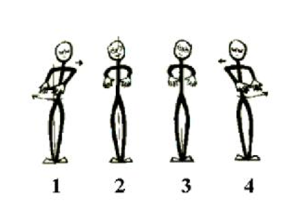
\includegraphics[height=5cm]{images/Exam_cli/Romberg.png}
    \caption{Illustration du test de Romberg}
    \label{fig:test_de_romberg}
\end{figure}


\begin{itemize}
    \item Le test de piétinement de Fukuda
\end{itemize}

Lors de ce test, le sujet doit reproduire un semblant de piétinement à raison d’un pas/seconde en levant le genou d’environ 45° et en maintenant les bras tendus vers l’avant. Il est invité à marcher sur place 50 fois, en levant les genoux bien hauts.
Afin d’obtenir de bon résultats, le test nécessite la mise en place de nombreuses précautions :  L'absence de sources sonores ou lumineuse, une élévation des cuisses à environ 45°, une fréquence approximative de 80 pas par minute, la position primaire des yeux à l'occlusion, la tête en position neutre puis tournée vers le côté droit puis gauche, si possible pieds nus, la mâchoires en position de posture mandibulaire après déglutition soit les dents qui ne se touchent pas.
Tout individu normal, piétinant sur place les yeux fermés, tourne sur lui-même seulement de 20° à 30° maximum en une cinquantaine de pas.

Ici, on peut observer :
\begin{itemize}
    \item 1.La tête tournée vers la gauche, l’individu dévie vers la droite.
    \item 2.La tête droite, un sujet normal lorsqu’il marque le temps, ne sort pas de la zone hachurée.
    \item 3.La tête tournée vers la droite, L’individu s’écarte vers la gauche.
\end{itemize}



\begin{figure}[H]
    \centering
    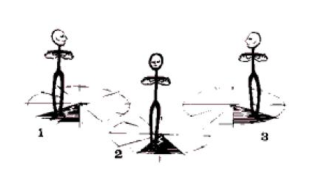
\includegraphics[height=5cm]{images/Exam_cli/pietinement.png}
    \caption{Illustration du test de piétinement de Fukuda} 
    \label{fig:test_de_Fukuda}
\end{figure}



\begin{itemize}
    \item Quelques alternatives :
    \begin{itemize}
        \item Test Unipodal 
        
        Ce test à pour objectif d’évaluer la stabilité statique du patient sur un seul appuie  afin d’identifier les individus présentant un faible équilibre, soit un risque accru de chute. Le but est de mettre en avant la proprioception  du patient et ainsi prouver l’intégrité fonctionnelle de son système postural. Le patient doit durant le test, se tenir sur une jambe, yeux ouverts, puis yeux fermés. Les paramètres stabilométriques mesurés via les oscillations permettent d’évaluer les capacités du patient à maintenir son équilibre.

\begin{figure}[H]
    \centering
    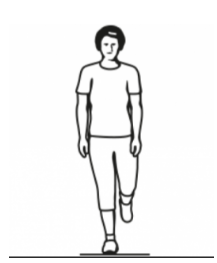
\includegraphics[height=5cm]{images/Exam_cli/Unipodal.png}
    \caption{Illustration du test Unipodal} 
    \label{fig:test_de_Unipodal}
\end{figure}
        
        \item   Test de la Perturbation Visuelle 
        Le test de la perturbation visuelle à pour but d’étudier la dépendance visuelle d’un sujet pour son équilibre. Le patient fixe alors un point visuel stable et un perturbation (changement du champ visuel, stimulation lumineuse) est introduite afin d'observer les compensations posturales de l’individu. 
    \end{itemize}
\end{itemize}

\newpage
\section{Annexe 2 : Méthodes d'analyse}

\subsection{Analyse spatio-temporelle}

L'analyse spatio-temporelle permet de déterminer la qualité de l'équilibre orthostatique. 
Elle reflète la capacité du corps d'un patient à maintenir un bon équilibre en position stationnaire droite. 
Le signal étudié est la représentation temporelle de la trajectoire du CdM en position statique debout sur une plateforme statique. 
Il est important de rappeler que ces méthodes sont directement applicables avec le CdP.

\subsubsection{Position moyenne du CdM}

\begin{equation}
  M_{AP} = \frac{1}{n} \sum_{n=1}^N \mbox{CdM}_{AP}(n) 
  \label{eq:M_AP}
\end{equation}

\begin{equation}
  M_{ML} = \frac{1}{n} \sum_{n=1}^N \mbox{CdM}_{ML}(n) 
  \label{eq:M_ML}
\end{equation}

La position moyenne du CdM représente la moyenne de l'ensemble des positions successives du CdM. 
Elle est calculée pour deux types de mouvements : les déplacements médio-latéraux ($M_{ml}$), ainsi que pour les déplacements antéro-postérieurs ($M_{ap}$).

Plus les valeurs sont basses, plus la qualité de l'équilibre est bonne.
La position moyenne est régulièrement couplée à l'écart-type, afin de pouvoir les situer l'un par rapport à l'autre, et ainsi donner une idée de la dispersion autour de la moyenne.

\subsubsection{Vitesse moyenne du CdM}

\begin{equation}
  L_{AP} = \sum_{n=1}^{N-1} \left| \mbox{CdM}_{AP}(n+1) - \mbox{CdM}_{AP}(n) \right|
  \label{eq:L_AP}
\end{equation}

\begin{equation}
  L_{ML} = \sum_{n=1}^{N-1} \left| \mbox{CdM}_{ML}(n+1) - \mbox{CdM}_{ML}(n) \right|
  \label{eq:L_ML}
\end{equation}

La mesure des longueurs des déplacements du centre de masse sur les deux axes (équations \ref{eq:L_AP} et \ref{eq:L_ML}) permettent d'estimer l'énergie dépensée pour la régulation de la posture orthostatique.

\begin{equation}
    MV_{AP} = \frac{L_{AP}}{T}
    \label{eq:MV_AP}
\end{equation}

\begin{equation}
    MV_{AP} = \frac{L_{ML}}{T}  
    \label{eq:MV_ML}    
\end{equation}

Les vitesses ainsi calculées représentent alors le tracé total en fonction du temps. 
Une vitesse élevée signifie un mauvais équilibre. 
Elles peuvent aussi renseigner sur la consommation d'énergie.

\subsubsection{Valeur quadratique moyenne (RMS pour root mean square}

\begin{equation}
    RMS_{AP} =\sqrt{  \frac{\sum_{n=1}^{N} \left (\text{CoM}_{AP}(n) \right)^2 }{N}}
    \label{eq:RMS_AP}
\end{equation}

\begin{equation}
    RMS_{ML} =\sqrt{  \frac{\sum_{n=1}^{N} \left (\text{CoM}_{ML}(n) \right)^2 }{N}}
    \label{eq:RMS_ML}
\end{equation}

Le calcul des moyennes quadratiques des amplitudes de déplacement du CdM sur les deux axes définis précédemment permet de quantifier l'habileté à maintenir l'équilibre. 
Plus ces mesures sont basses, plus l'habileté est grande.

\subsubsection{Écart maximal}

\begin{equation}
  R_{AP}= max \left ( \text CoM_{AP} \right ) - min\left ( \text CoM_{AP} \right ) 
  \label{eq:R_AP}
\end{equation}

\begin{equation}
  R_{ML}= max \left ( \text CoM_{ML} \right ) - min\left ( \text CoM_{ML} \right )   
  \label{eq:R_ML}
\end{equation}


L'écart maximal est la différence entre la position maximale et minimale du CdM et est défini suivant les deux axes AP et ML.
Une augmentation d'une de ces valeurs peut être interprétable en une baisse de la capacité à maintenir l'équilibre postural.

\subsubsection{Surface de l'ellipse de confiance (CEA)}

\begin{equation}
CEA= 6\pi \sqrt{ \left ( \frac{\sum_{n=1}^{N} \left (\text{CoM}_{AP}(n) \right)^2 \times \sum_{n=1}^{N} \left ( \text{CoM}_{ML}(n) \right)^2}{N^2} \right ) - \left (\frac{\sum_{n=1}^N \text{CoM}_{AP} \times CoM_{ML}}{N} \right)^2}
\label{eq:CEA}
\end{equation}

La surface de l'ellipse de confiance regroupe un certain pourcentage du statokinésigramme (en cm2), ici 95\%. 
Cette intervalle de confiance peut varier selon les pratiques ou les habitudes (certains praticiens utilisent une surface d'ellipse de confiance de 90\% par exemple). 
Plus précisément, c'est l'évolution du périmètre de l'ellipse qui est étudiée. 
Plus ce périmètre est grand, et plus l'équilibre est mauvais.

\begin{figure}[H]
    \centering
    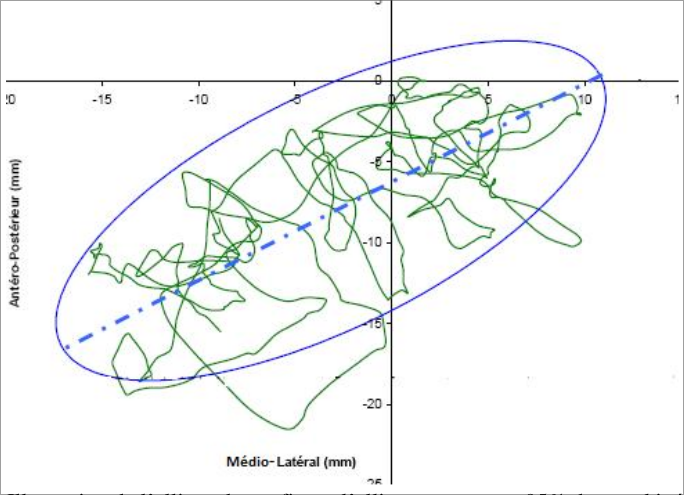
\includegraphics[height=8cm]{images/methode/ellipse_confiance_95.png}
    \caption{Illustration de l'ellipse de confiance (à 95\% du statokinésigramme)}\label{fig:ellipse_confiance}
\end{figure}

\subsubsection{Quotient de Romberg}

\begin{equation}
  QR = \frac{\text{CEA}_{\text{YF}}}{\text{CEA}_{\text{YO}}}
  \label{eq:QR}
\end{equation}

Ce quotient entre la valeur de CEA yeux fermés et la valeur de CEA yeux ouverts permet de mettre en évidence le rôle de la vision dans le contrôle de la posture. 
Une valeur élevée de ce quotient indique une dépendance visuelle accrue dans le maintien de l'équilibre.

\subsection{Analyse spectrale}

L'analyse spectrale se situe dans le domaine fréquentiel.
Le spectre d'un signal permet d'extraire les différentes composantes présentes dans le signal. 
L'analyse spectrale permet de différencier les différents mécanismes utilisés dans le maintien de l'équilibre en position statique.
Le spectre de fréquence est obtenu en appliquant la transformation de Fourier, principe mathématique, à un signal temporel. 
L'analyse spectrale permet de mettre en évidence l'aspect dynamique du contrôle de la posture orthostatique.

\subsubsection{Fréquence moyenne ou centroïdale}

\begin{equation}
  \text{FM}_{\text{AP}} = \frac{\text{MV}_{\text{AP}}}{4\cdot\sqrt{2}\cdot\text{M}_{\text{AP}}}
  \label{eq:FM_AP}
\end{equation}

\begin{equation}
  \text{FM}_{\text{ML}} = \frac{\text{MV}_{\text{ML}}}{4 \cdot \sqrt{2} \cdot \text{M}_{\text{ML}}}
  \label{eq:FM_ML}
\end{equation}

La fréquence moyenne est le paramètre qui permet d'étudier le temps nécessaire au mouvement analysé pour revenir dans une position identique. 
Son calcul passe par l'analyse de la distribution fréquentielle des amplitudes.

\subsubsection{Puissance moyenne de la densité spectrale}

\begin{equation}
  P_{\text{Per}}(f) = \frac{1}{N T_e} \left| \sum_{n=0}^{N-1} x(nT_e)e^{-j2\pi n T_e f} \right|^2
  \label{eq:P_Per}
\end{equation}

La puissance moyenne de la densité spectrale correspond à la quantité d'énergie contenue dans les oscillations du CdP.
Généralement, une faible puissance indique une stabilité correcte, avec peu d'ajustements nécessaires.
Une puissance élevée indiquerait des oscillations plus importantes, et donc une instabilité.

Le processus consiste à :
\begin{itemize}
    \item \textbf{Appliquer la transformée de Fourier discrète (TFD)} au signal $x(nT_e)$ pour transformer le signal temporel en un spectre fréquentiel.
    \item \textbf{Calculer la puissance} à chaque fréquence en prenant le carré du module de la TFD.
    \item \textbf{Normaliser} par $\frac{1}{N T_e}$ pour obtenir une estimation de la DSP, qui représente la distribution de la puissance du signal dans le domaine fréquentiel.
\end{itemize}

Cette estimation permet de voir quelles fréquences contiennent le plus de puissance dans le signal, ce qui est crucial pour l'analyse fréquentielle dans divers domaines, comme la stabilographie, le traitement du signal audio, et d'autres types d'analyse de séries temporelles.

On calcule alors l’estimateur de Welch à partir du périodogramme calculé comme ci-dessus.

\begin{equation}
  P_{Welch}(f) = \frac{1}{L} \sum_{l=1}^{L-1}P_l(f)
  \label{P_Welch}
\end{equation}

\begin{equation}  
  P_l(f) = \left( \frac{1}{K}\right) \left |\sum_{n=0}^{K-1} x(n+lK) w(n) e^{-j2\pi nf} \right |^2
  \label{eq:Pl_f}
\end{equation}

L'estimateur de Welch est une amélioration du périodogramme classique pour estimer la densité spectrale de puissance (DSP) d'un signal. 
Il permet de réduire la variance de l'estimation de la DSP, ce qui en fait une méthode plus robuste pour analyser des signaux bruités ou irréguliers. 
Voici ce que l'estimateur de Welch apporte par rapport au périodogramme simple :

\textbf{1. Réduction de la variance :}
La périodogramme classique a tendance à être un estimateur à variance élevée, c'est-à-dire que ses résultats peuvent fluctuer de manière importante d'un signal à l'autre, même si ceux-ci ont une structure similaire. 
Cela peut rendre l'analyse spectrale moins fiable. 
L'estimateur de Welch réduit cette variance en moyennant plusieurs estimations de la DSP obtenues à partir de segments du signal.

\textbf{2. Segmenter et fenêtrer le signal :}
L'algorithme de Welch divise le signal en plusieurs segments qui se chevauchent partiellement (typiquement de 50\%), et applique une fenêtrage à chaque segment (souvent une fenêtre de Hanning ou de Hamming). 

Ce processus présente plusieurs avantages:
\begin{itemize}
    \item \textbf Segmenter le signal permet de découper le signal en morceaux plus petits, ce qui donne plusieurs petites estimations de la DSP au lieu d'une seule estimation basée sur tout le signal.
    \item \textbf Fenêtrer chaque segment aide à atténuer les discontinuités aux bords des segments, qui pourraient introduire des artefacts dans le domaine fréquentiel, comme des fuites spectrales.
\end{itemize}

\textbf{3. Chevauchement des segments}
Les chevauchements des segments (souvent 50\%) augmentent la quantité d'information utilisée pour chaque estimation locale, améliorant ainsi la stabilité de l'estimation globale. 
Cela permet d'améliorer la résolution fréquentielle tout en conservant une meilleure estimation des puissances.

\textbf{4. Moyenne des DSP :}
Après avoir calculé la transformée de Fourier et le périodogramme pour chaque segment, l'algorithme de Welch prend la moyenne des densités spectrales de puissance (DSP) obtenues. 
Cette moyenne réduit la variance des résultats et améliore la stabilité de l'estimation. 
Le fait de mesurer plusieurs estimations atténue également les fluctuations dues au bruit.

L'estimateur de Welch apporte certains avantages : 
\begin{itemize}
    \item  \textbf{Variance plus fiable} : Comme chaque périodogramme segmenté est moyenné, l'estimateur de Welch a une variance significativement plus fiable que le périodogramme classique, offrant une estimation plus fiable.
    \item \textbf{Meilleure résolution fréquentielle} : Même si chaque segment est plus court que le signal original, l'utilisation du chevauchement permet de conserver une bonne résolution fréquentielle tout en réduisant la variance.
    \item  \textbf{Atténuation des fuites spectrales} : l'application d'une fenêtre sur chaque segment réduit les artefacts induits par les discontinuités aux bords du signal.
\end{itemize}

\begin{figure}[H]
    \centering
    \begin{subfigure}[b]{0.45\textwidth}
        \centering
        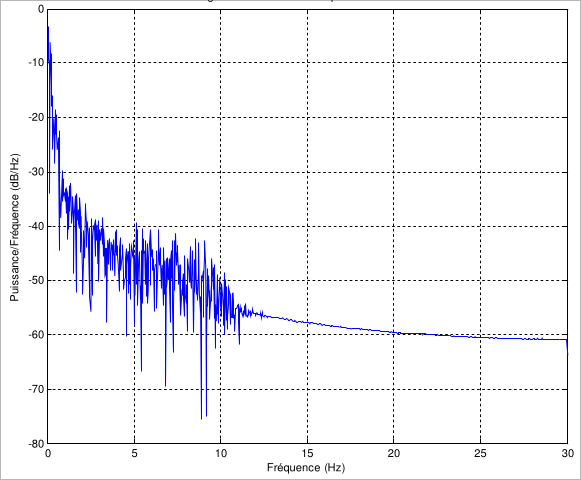
\includegraphics[height=5cm]{images/methode/periodogramme.png}
        \caption{Périodogramme de la densité spectrale de puissance}\label{fig:periodogramme}
    \end{subfigure}
    \begin{subfigure}[b]{0.45\textwidth}
        \centering
        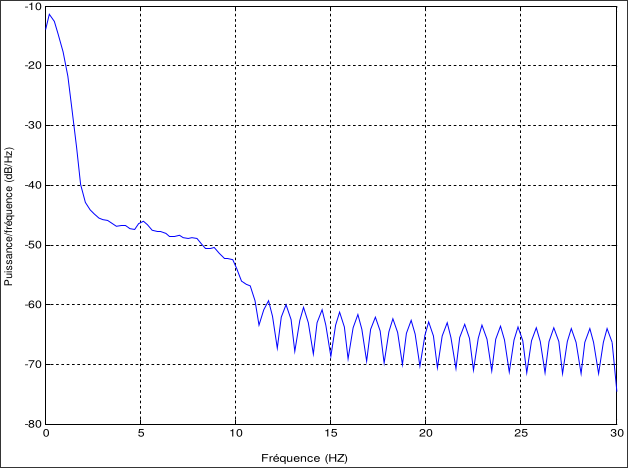
\includegraphics[height=5cm]{images/methode/welch.png}
        \caption{Estimation de Welch de la densité spectrale de puissance}\label{fig:welch}
    \end{subfigure}
    \caption{Comparaison entre le périodogramme et l'estimation de Welch de la densité spectrale de puissance}\label{fig:periodogramme_welch}
\end{figure}

\subsubsection{Pente du spectre de puissance}

Dans le cadre de la stabilographie, l’analyse du spectre dans le plan log-log permet de mieux comprendre les mécanismes de régulation posturale et de quantifier la stabilité ou l’instabilité en fonction des
fréquences des oscillations du CoP. La régression linéaire dans ce contexte permet d’estimer la pente du
spectre et de révéler les caractéristiques de contrôle postural, avec des applications potentielles pour le
diagnostic ou la suivi clinique des troubles de l’équilibre, ou encore pour la prévention des chutes chez
les personnes âgées.

Interprétation en stabilographie :

\begin{itemize}
    \item Stabilité posturale élevée : Lorsque la pente est fortement négative (par exemple au alentour de-2 ou plus), cela signifie que la puissance des oscillations posturales diminue rapidement avec la
    fréquence. Dans ce cas, les oscillations à basse fréquence dominent, ce qui suggère un contrôle
    postural efficace avec des ajustements lents et stables. Cela pourrait être typique chez un jeune
    adulte en bonne santé.

    \item Instabilité posturale : Lorsque la pente est moins négative (par exemple, autour de-1), cela peut
    signifier que les oscillations à haute fréquence contribuent davantage au contrôle postural. Ce type
    de spectre pourrait être observé chez des individus plus âgés ou des personnes ayant des troubles de
    l’équilibre, car il indique un contrôle moins stable et une plus grande participation des ajustements
    réflexes ou involontaires.
\end{itemize}


\begin{figure}[H]
    \centering
    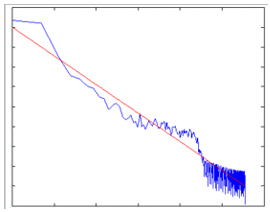
\includegraphics[height=5cm]{images/methode/analyse_spec_regre_lin.png}
    \caption{Analyse spectrale et régression linéaire}\label{fig:regression_lineaire}
\end{figure}

\newpage
\section{Annexe 3 : protocole complet}

\begin{figure}[H]
    \centering
    \caption{Plateforme imaginée}
    \begin{minipage}{0.3\textwidth}
        \centering
        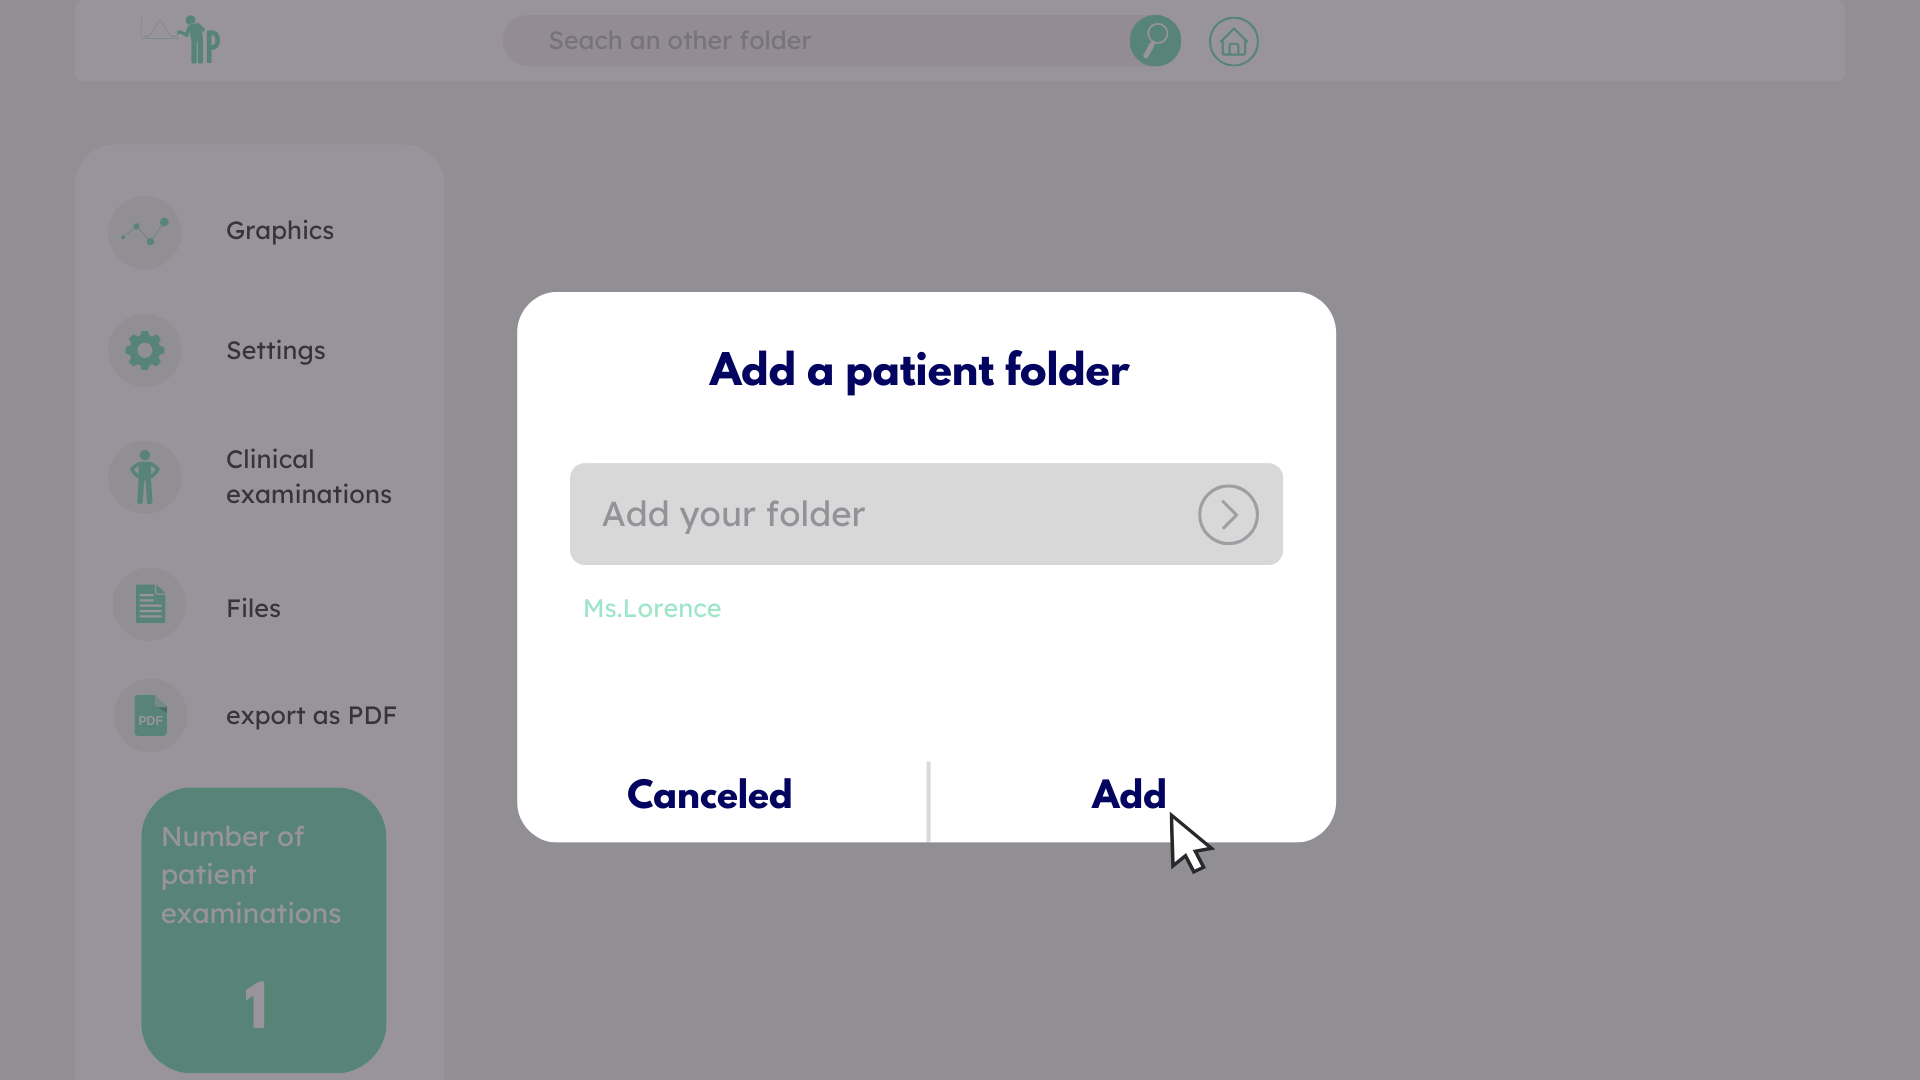
\includegraphics[width=\textwidth]{images/Prototype/1.png}
        \caption*{1}
    \end{minipage}
    \begin{minipage}{0.3\textwidth}
        \centering
        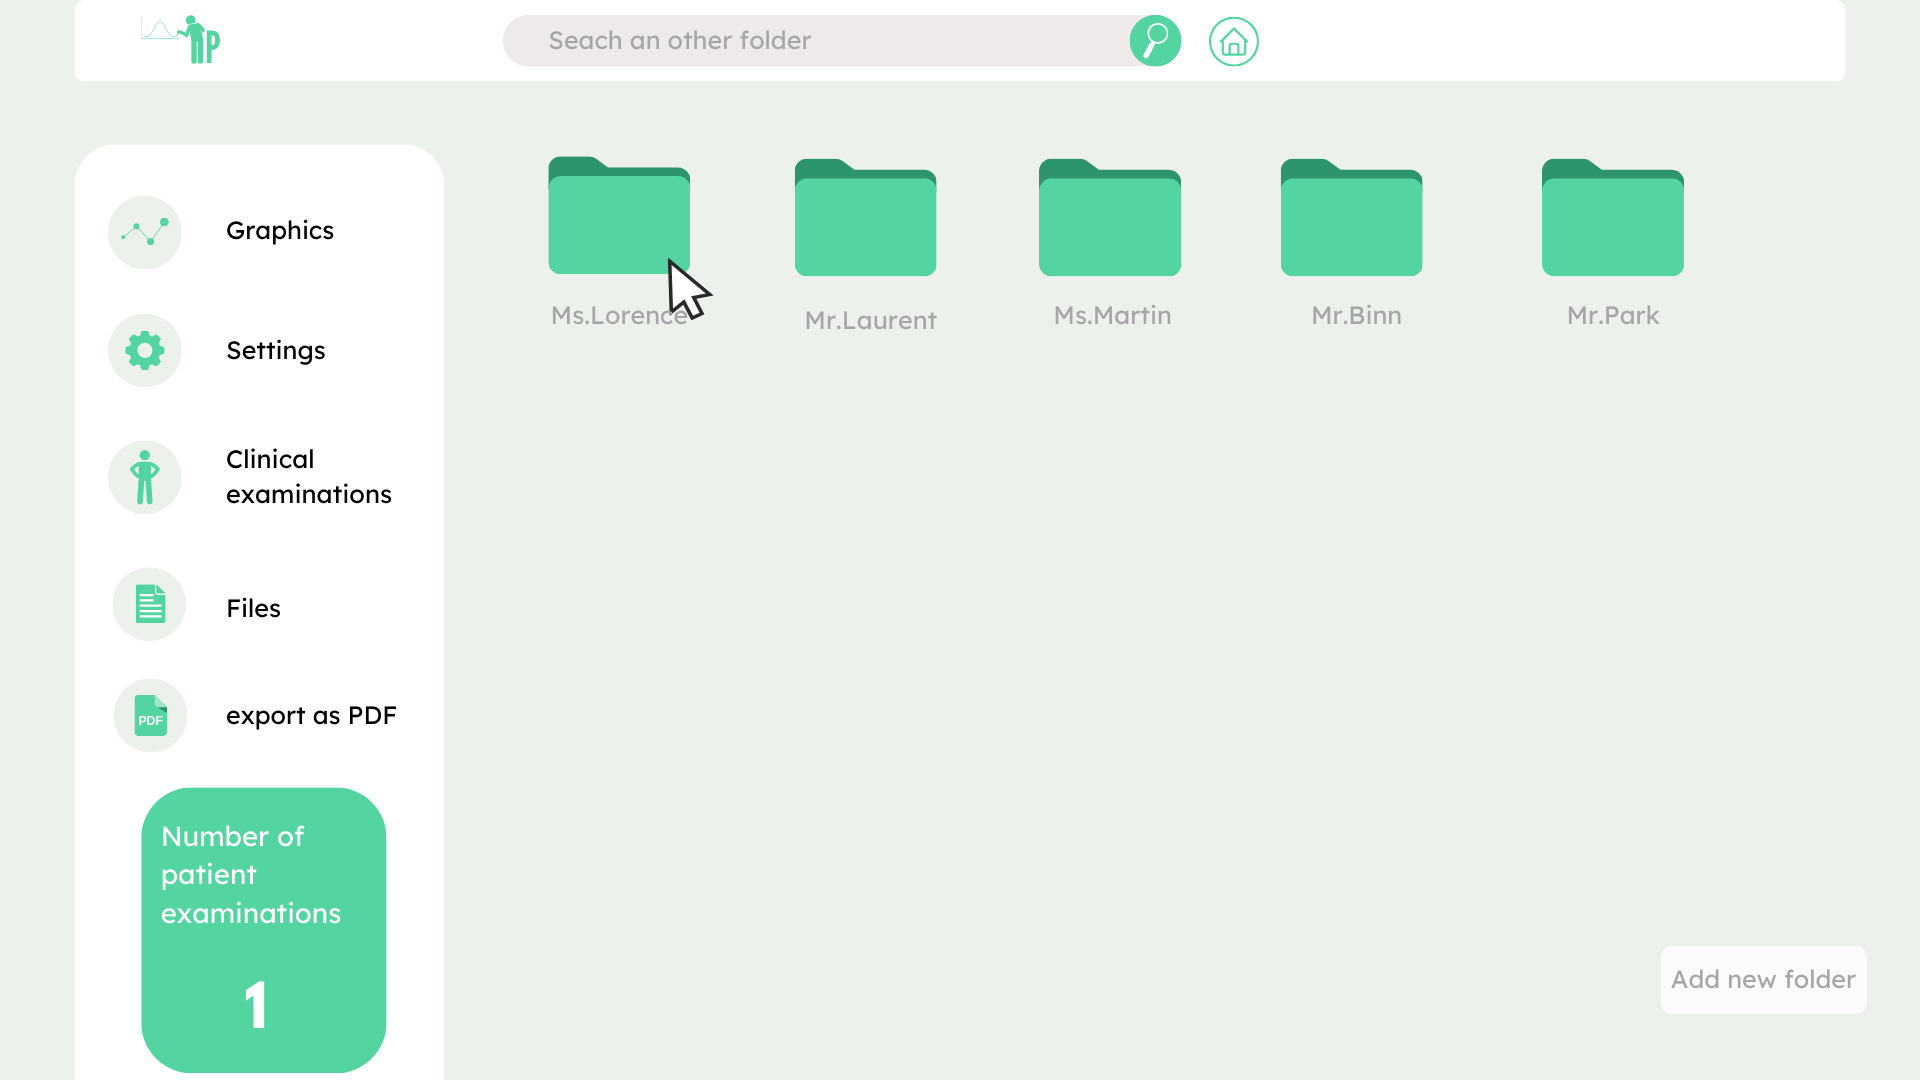
\includegraphics[width=\textwidth]{images/Prototype/Accueil de la plateforme de visualisation.png}
        \caption*{2}
    \end{minipage}
    \begin{minipage}{0.3\textwidth}
        \centering
        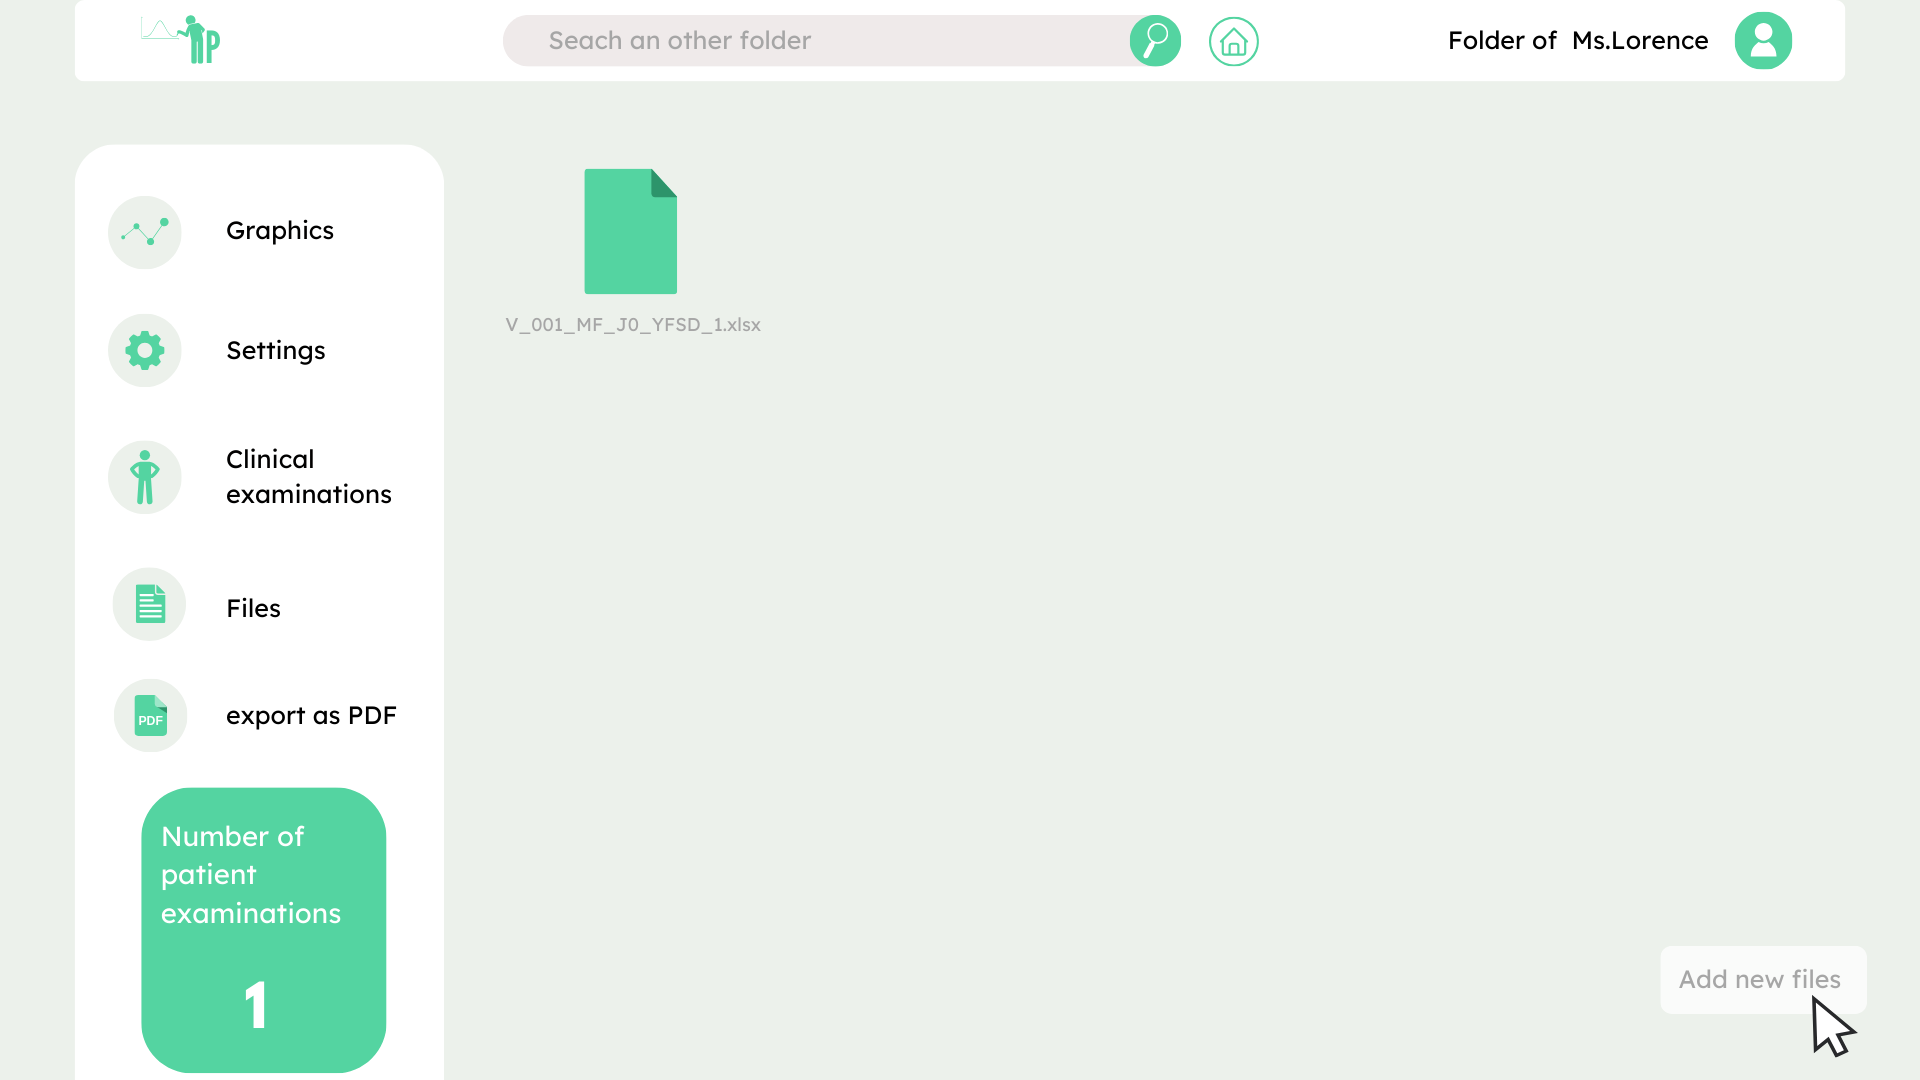
\includegraphics[width=\textwidth]{images/Prototype/3.png}
        \caption*{3}
    \end{minipage}
    \begin{minipage}{0.3\textwidth}
        \centering
        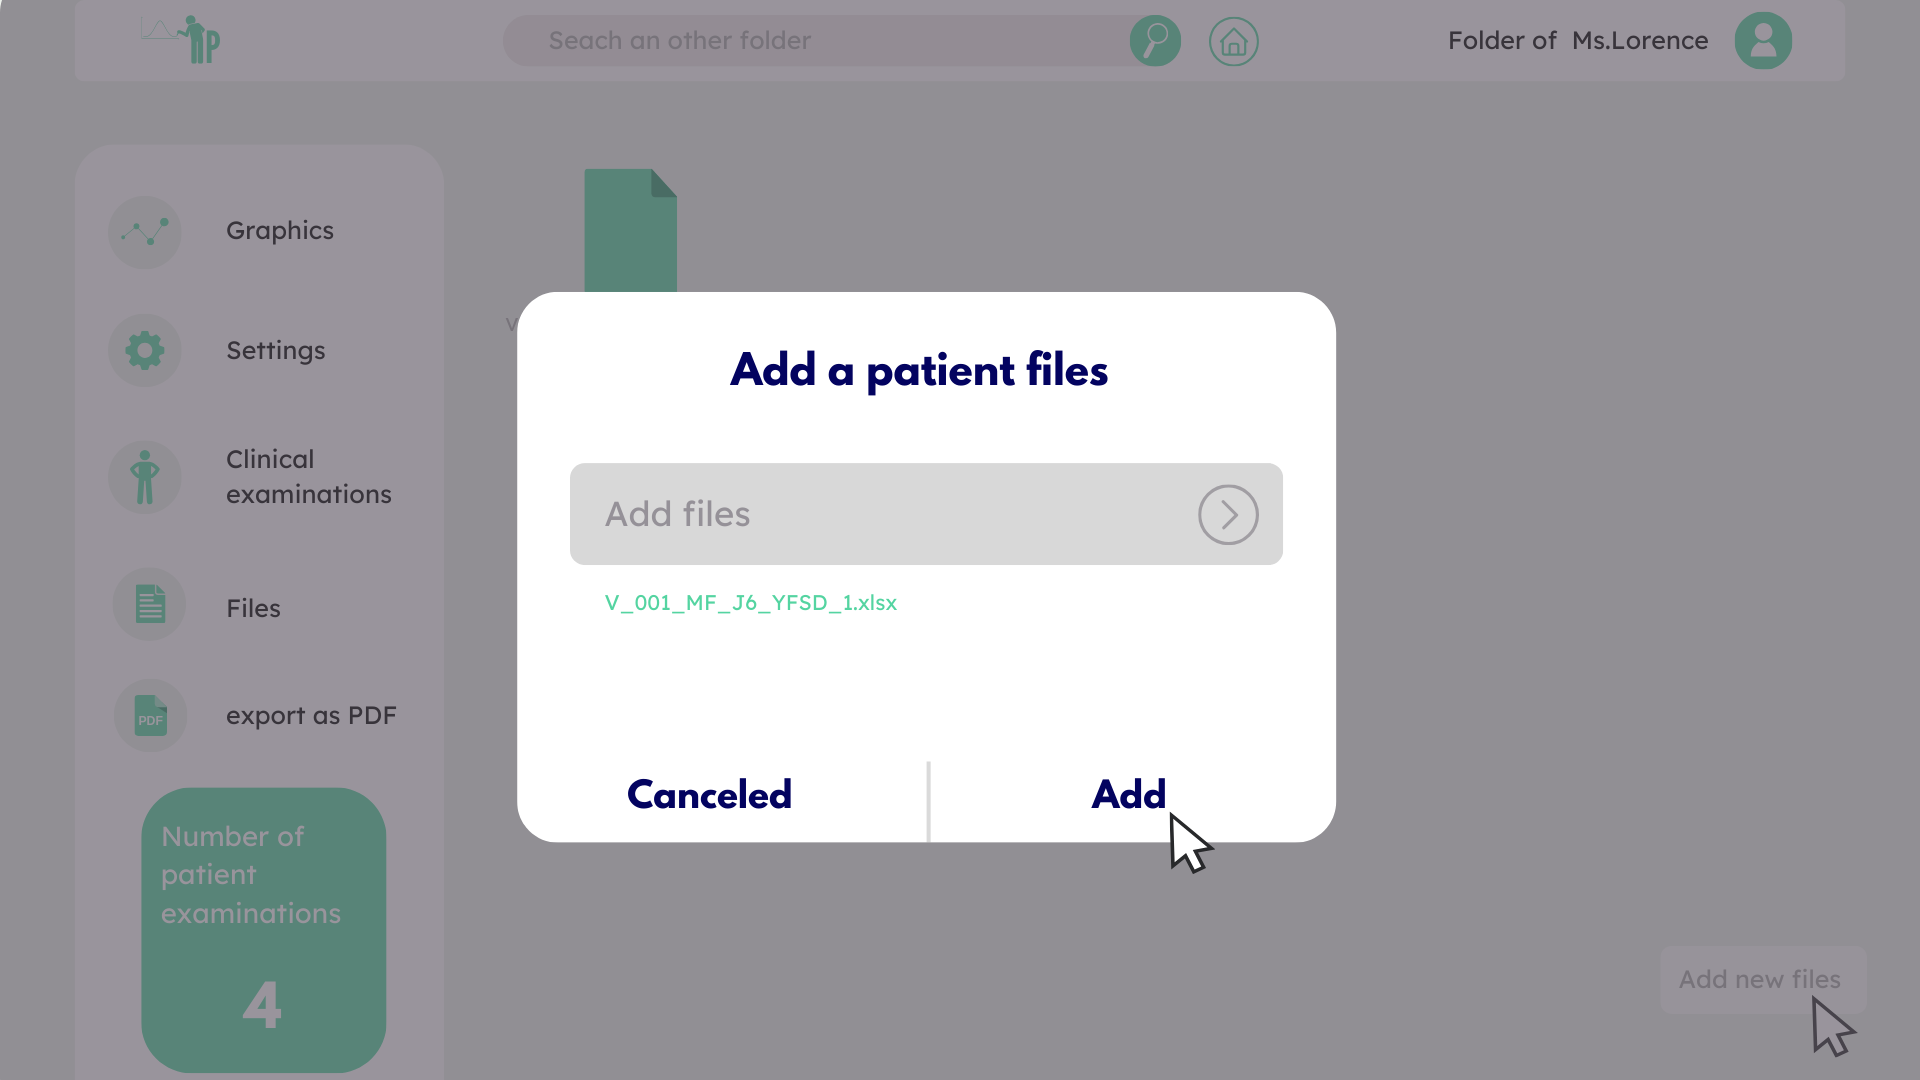
\includegraphics[width=\textwidth]{images/Prototype/4.png}
        \caption*{4}
    \end{minipage}
    \begin{minipage}{0.3\textwidth}
        \centering
        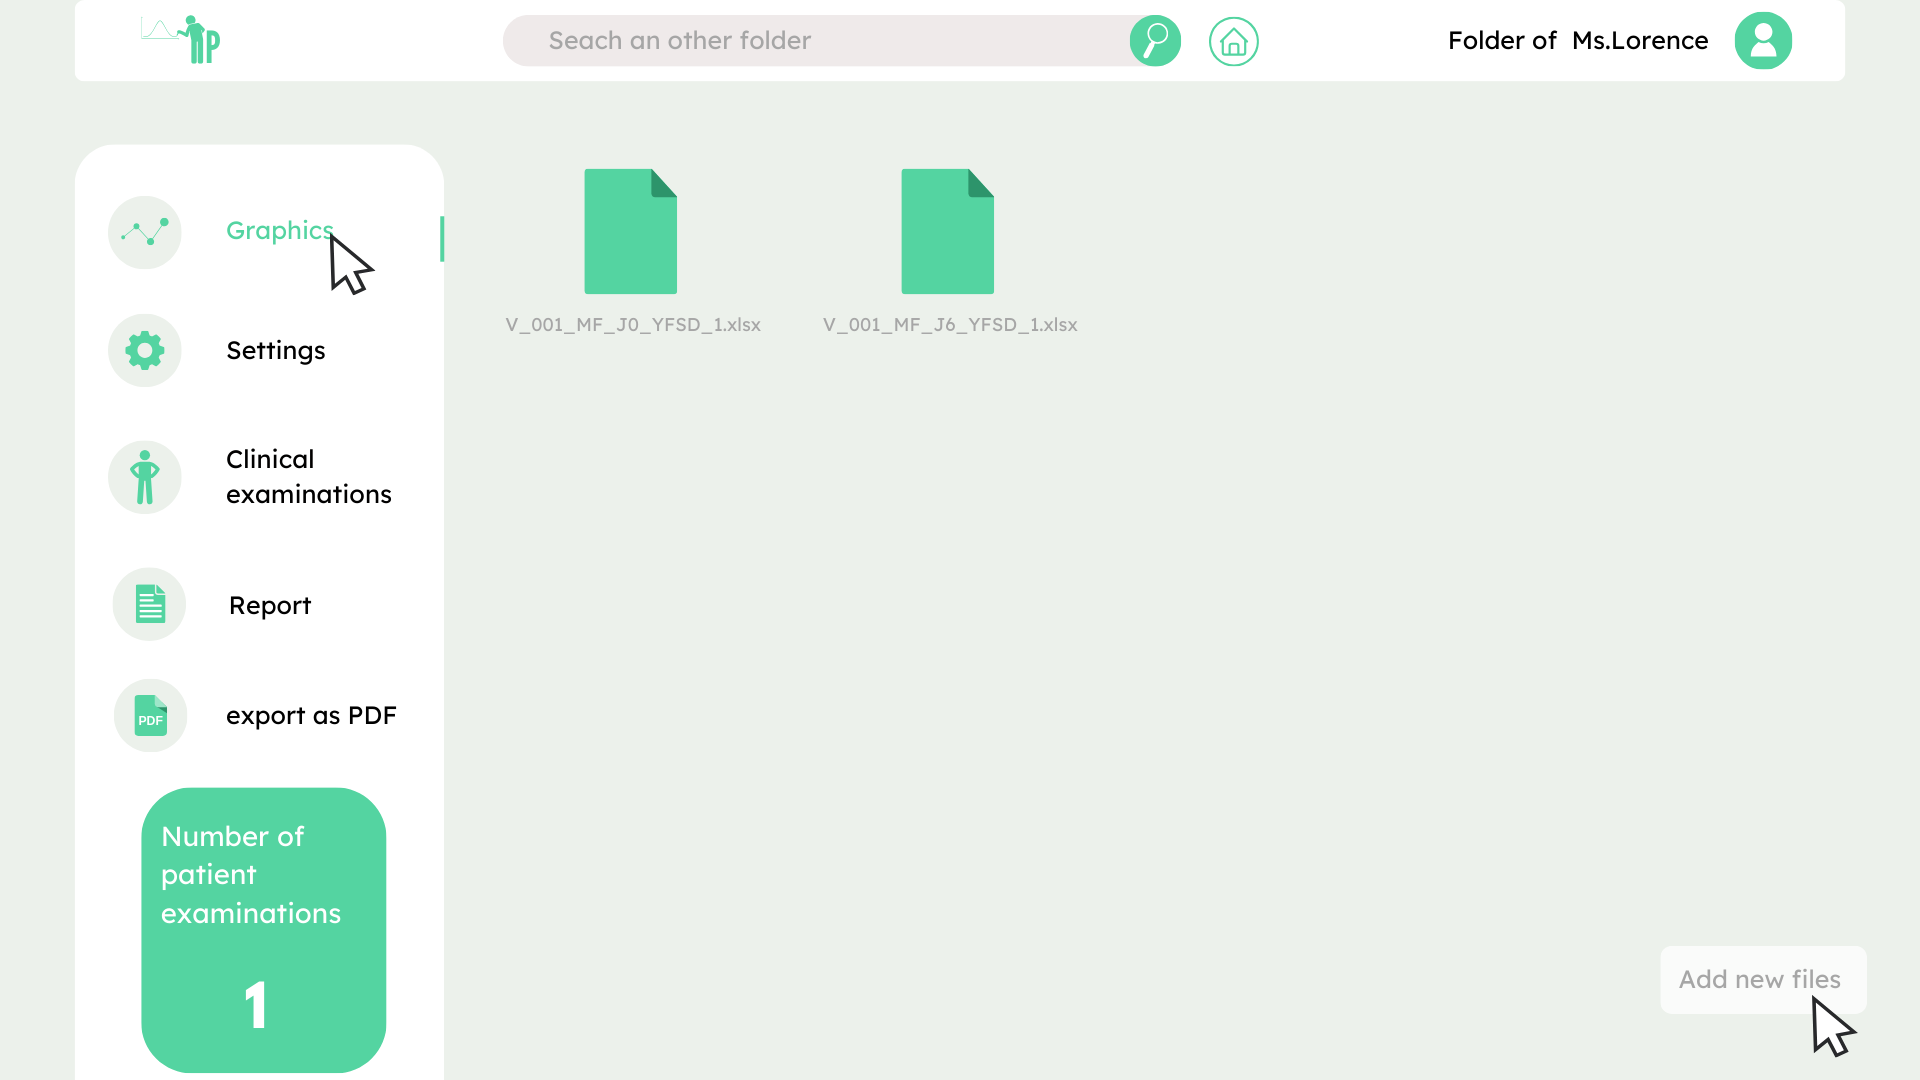
\includegraphics[width=\textwidth]{images/Prototype/5.png}
        \caption*{5}
    \end{minipage}
    \begin{minipage}{0.3\textwidth}
        \centering
        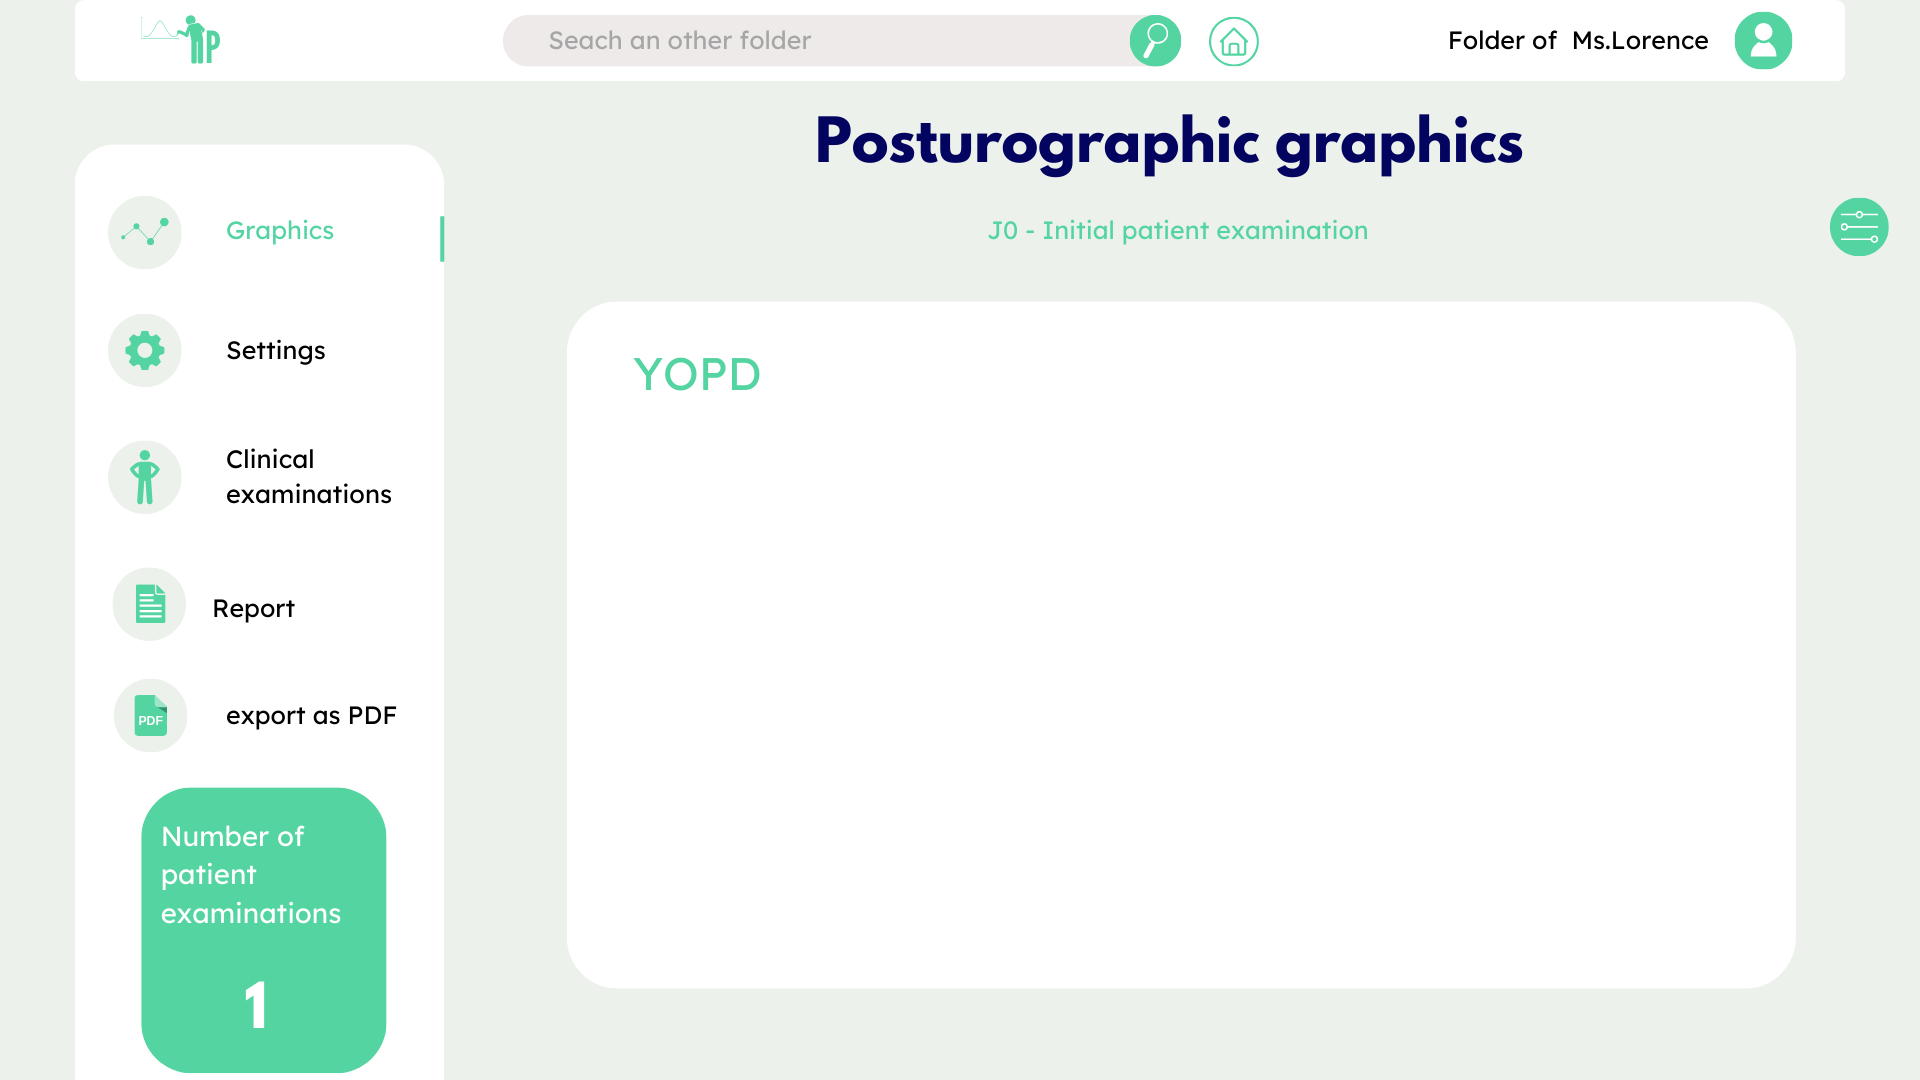
\includegraphics[width=\textwidth]{images/Prototype/6.png}
        \caption*{6}
    \end{minipage}
    \begin{minipage}{0.3\textwidth}
        \centering
        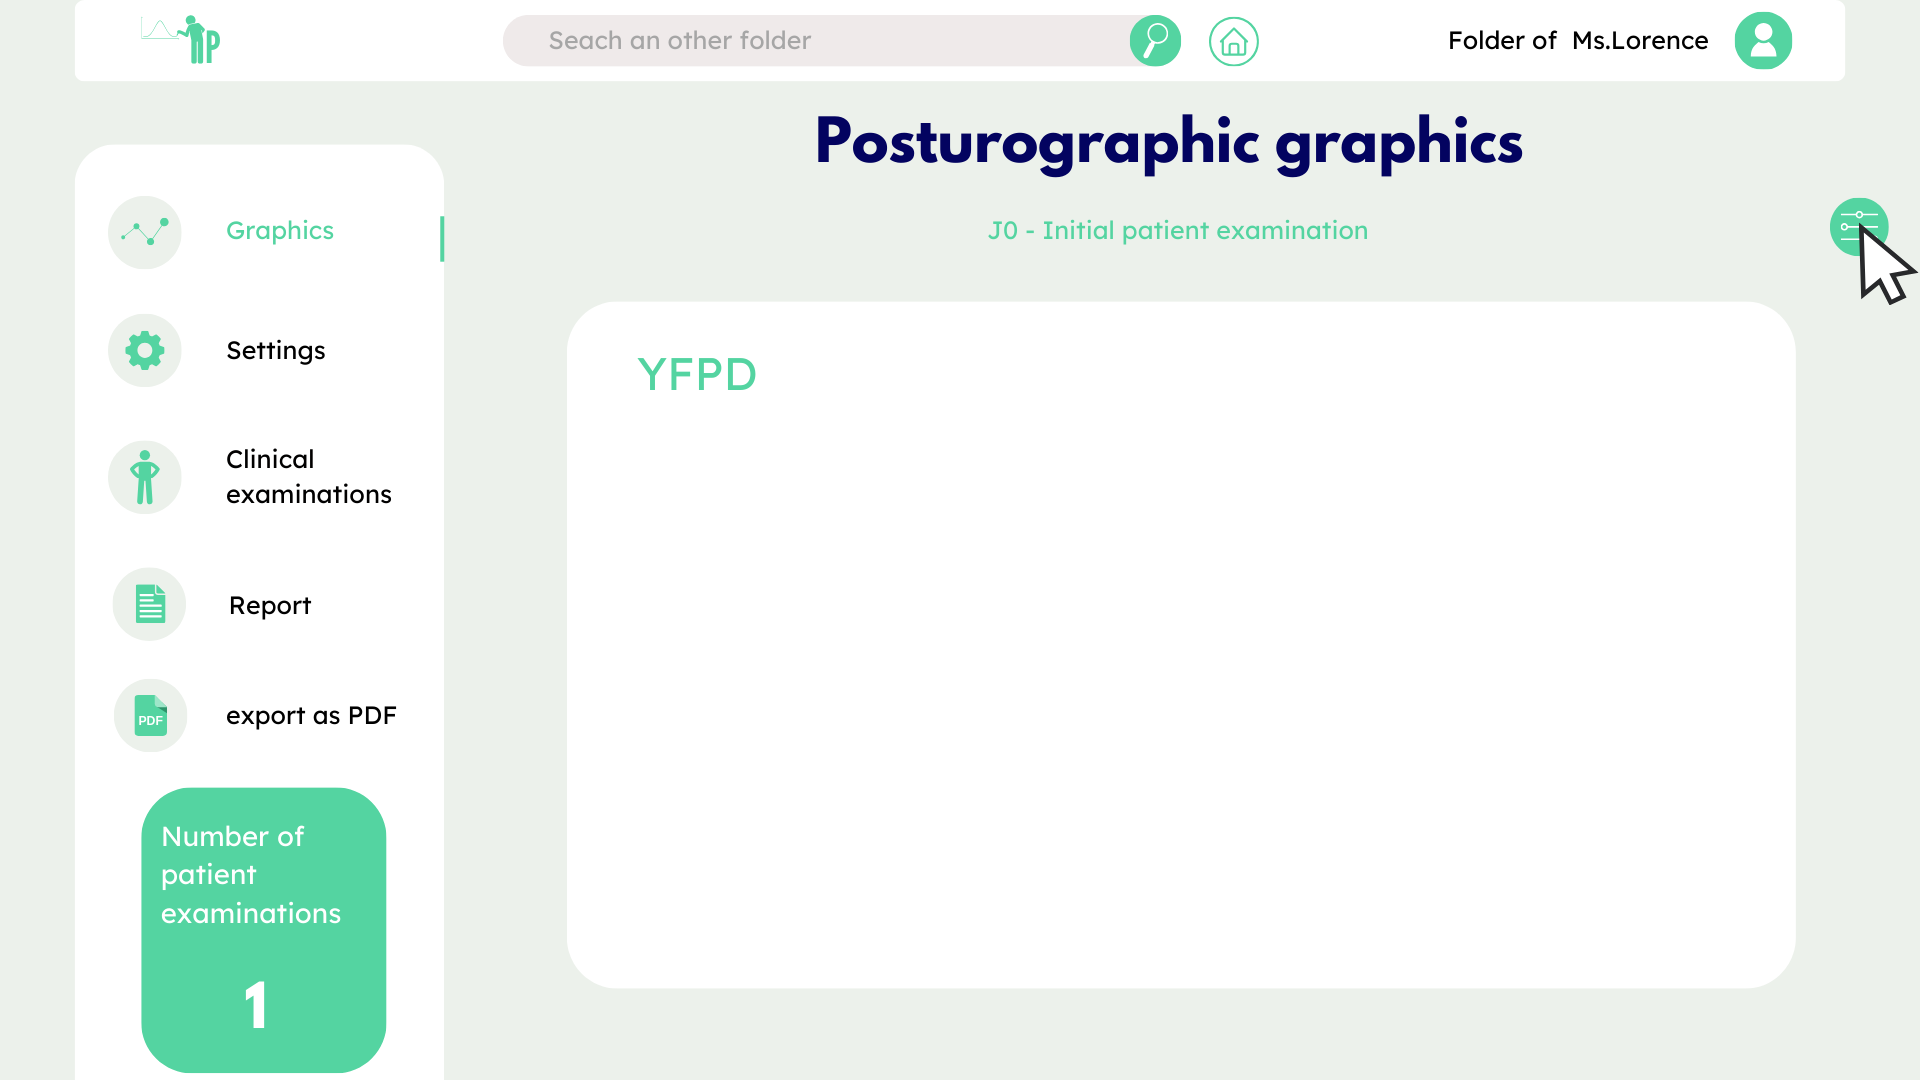
\includegraphics[width=\textwidth]{images/Prototype/7.png}
        \caption*{7}
    \end{minipage}
    \begin{minipage}{0.3\textwidth}
        \centering
        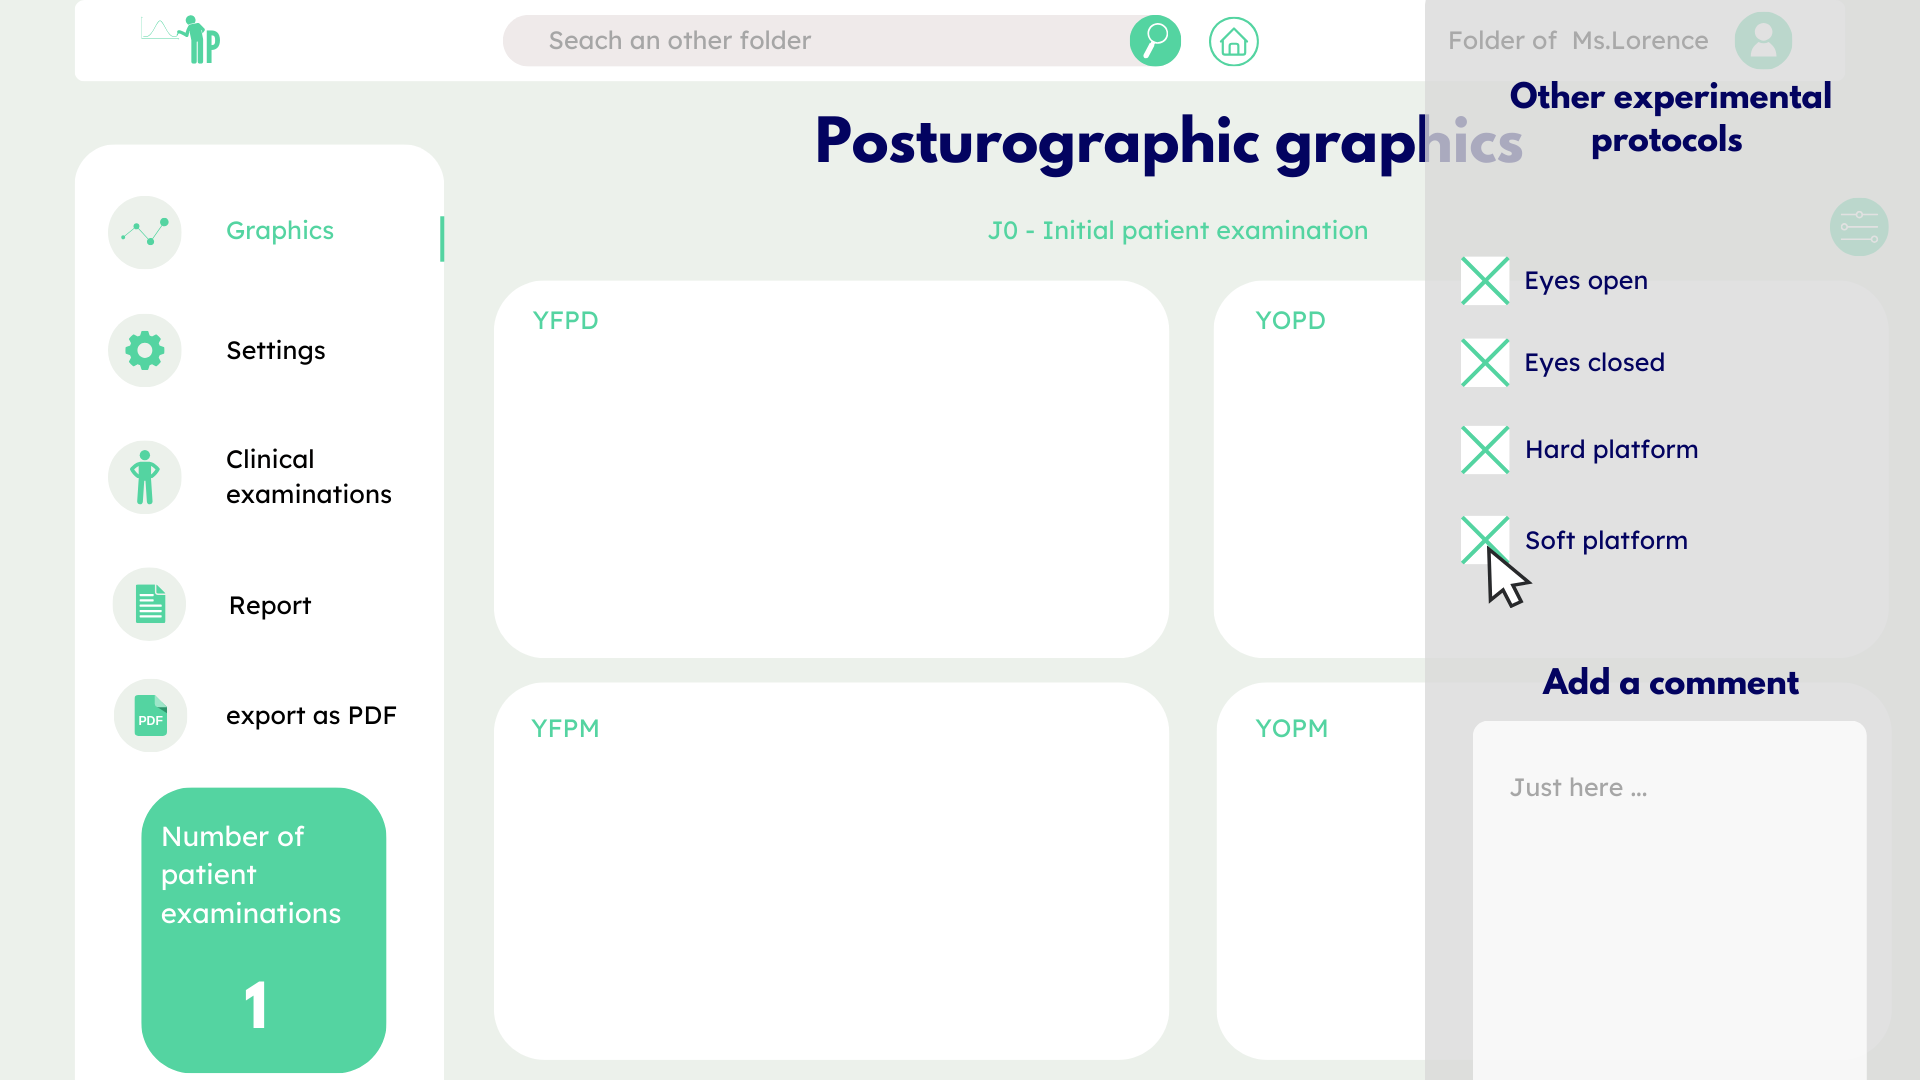
\includegraphics[width=\textwidth]{images/Prototype/Visualisation des données en fonction de différents protocoles expérimentaux.png}
        \caption*{8}
    \end{minipage}
    \begin{minipage}{0.3\textwidth}
        \centering
        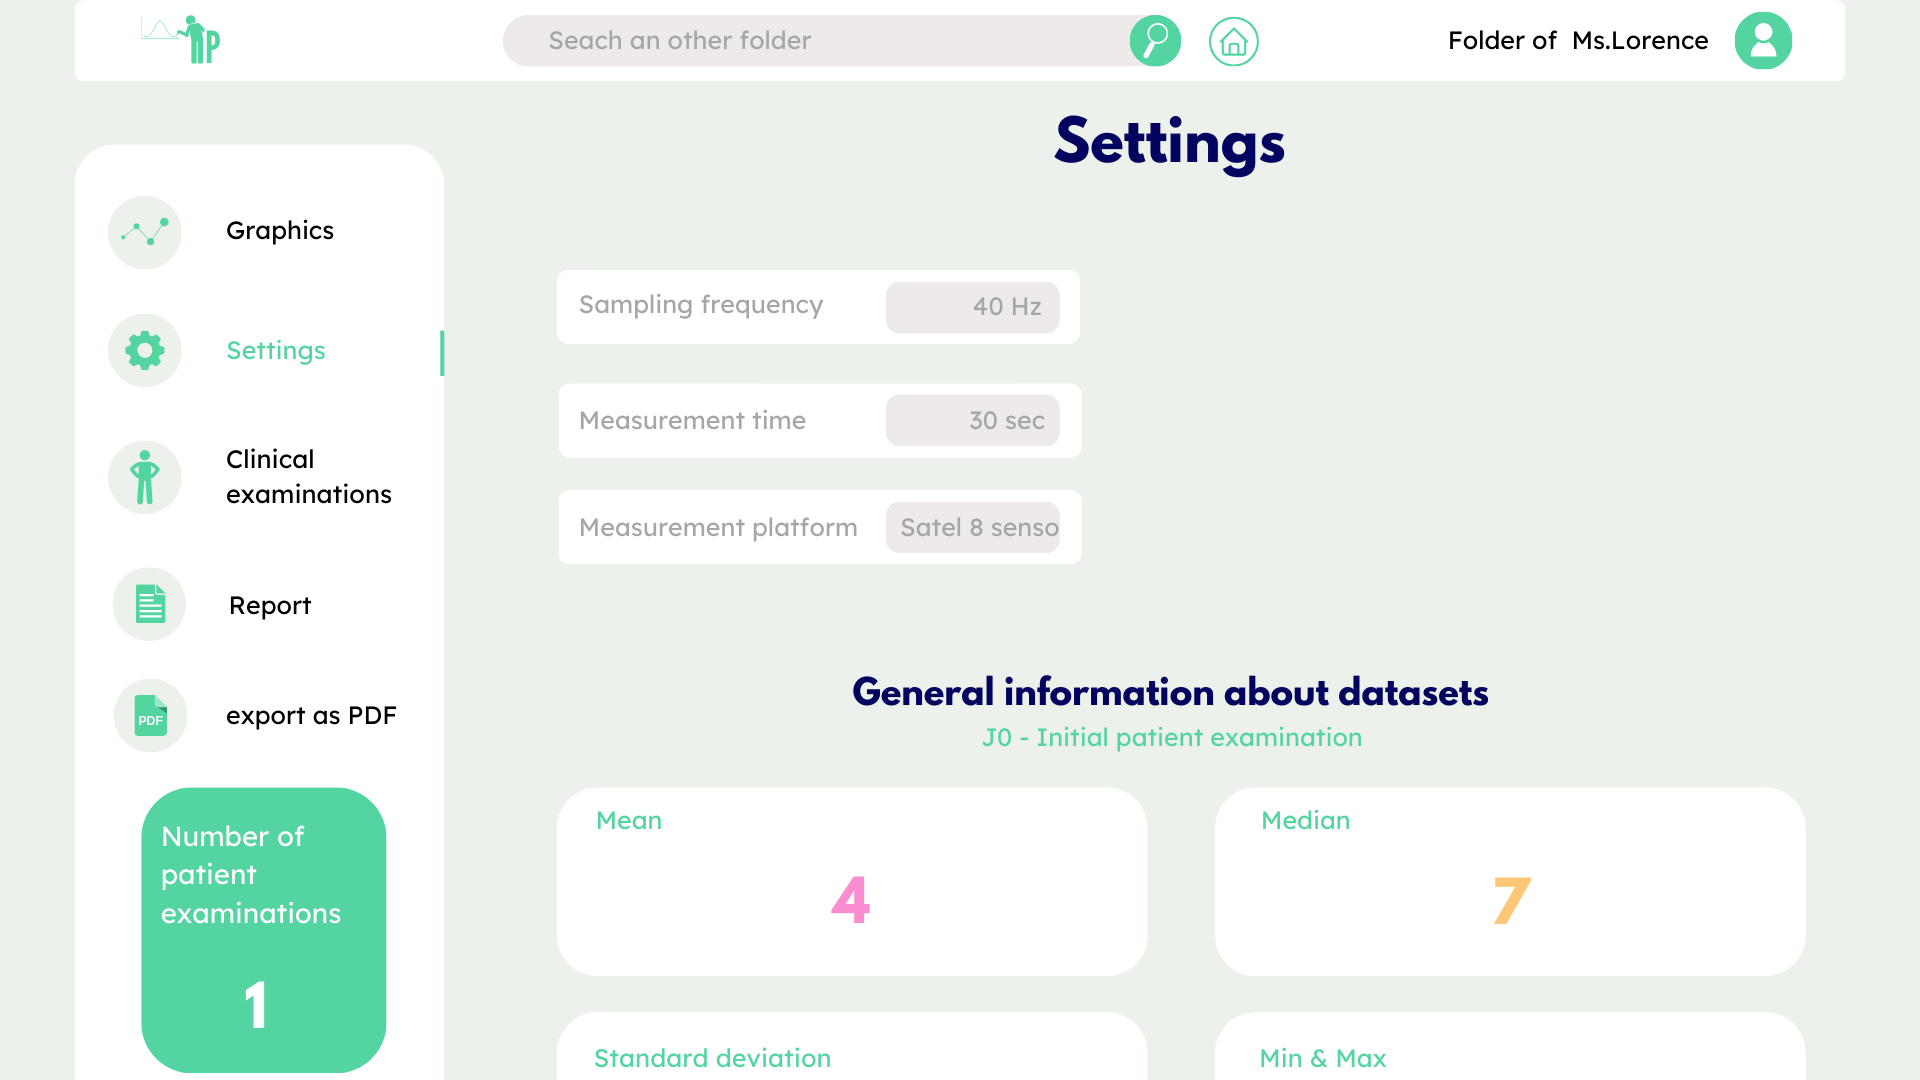
\includegraphics[width=\textwidth]{images/Prototype/visualiser des données clés du jeu de données étudié.png}
        \caption*{9}
    \end{minipage}
    \begin{minipage}{0.3\textwidth}
        \centering
        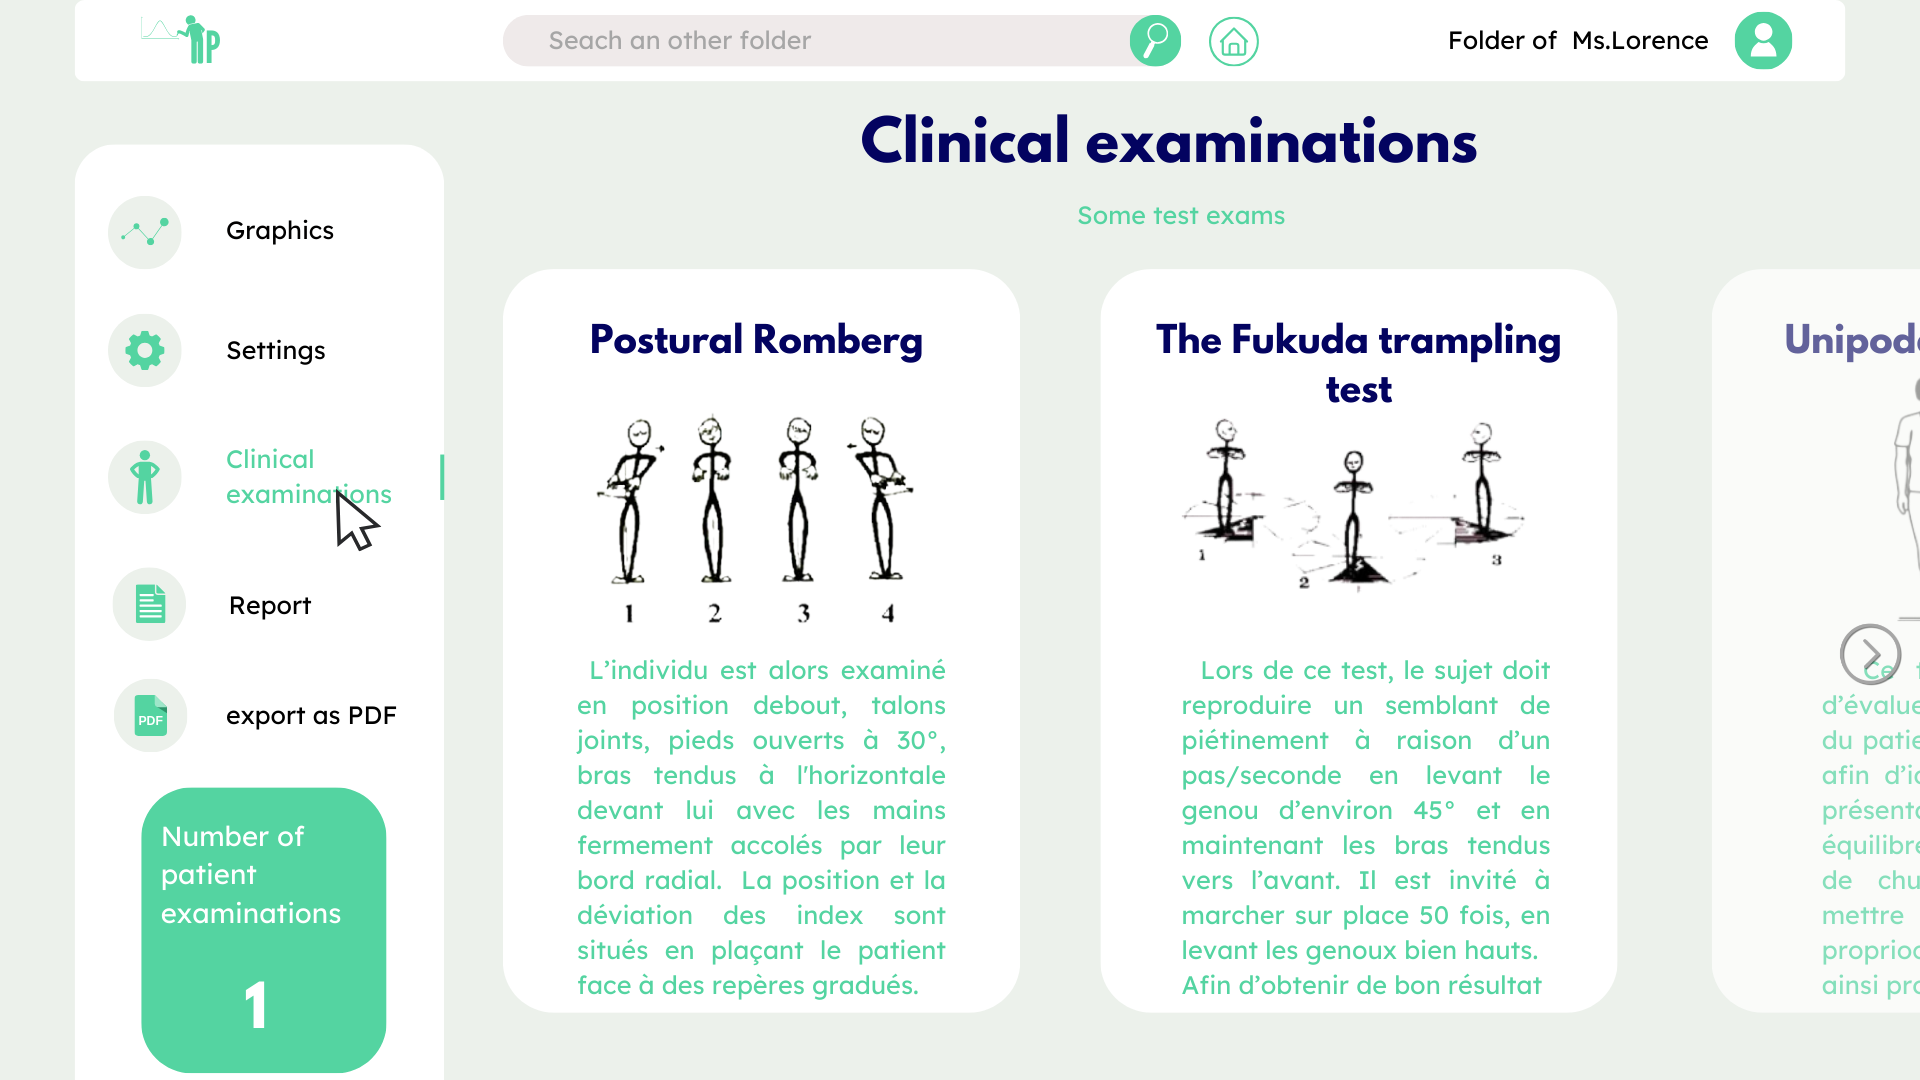
\includegraphics[width=\textwidth]{images/Prototype/10.png}
        \caption*{10}
    \end{minipage}
    \begin{minipage}{0.3\textwidth}
        \centering
        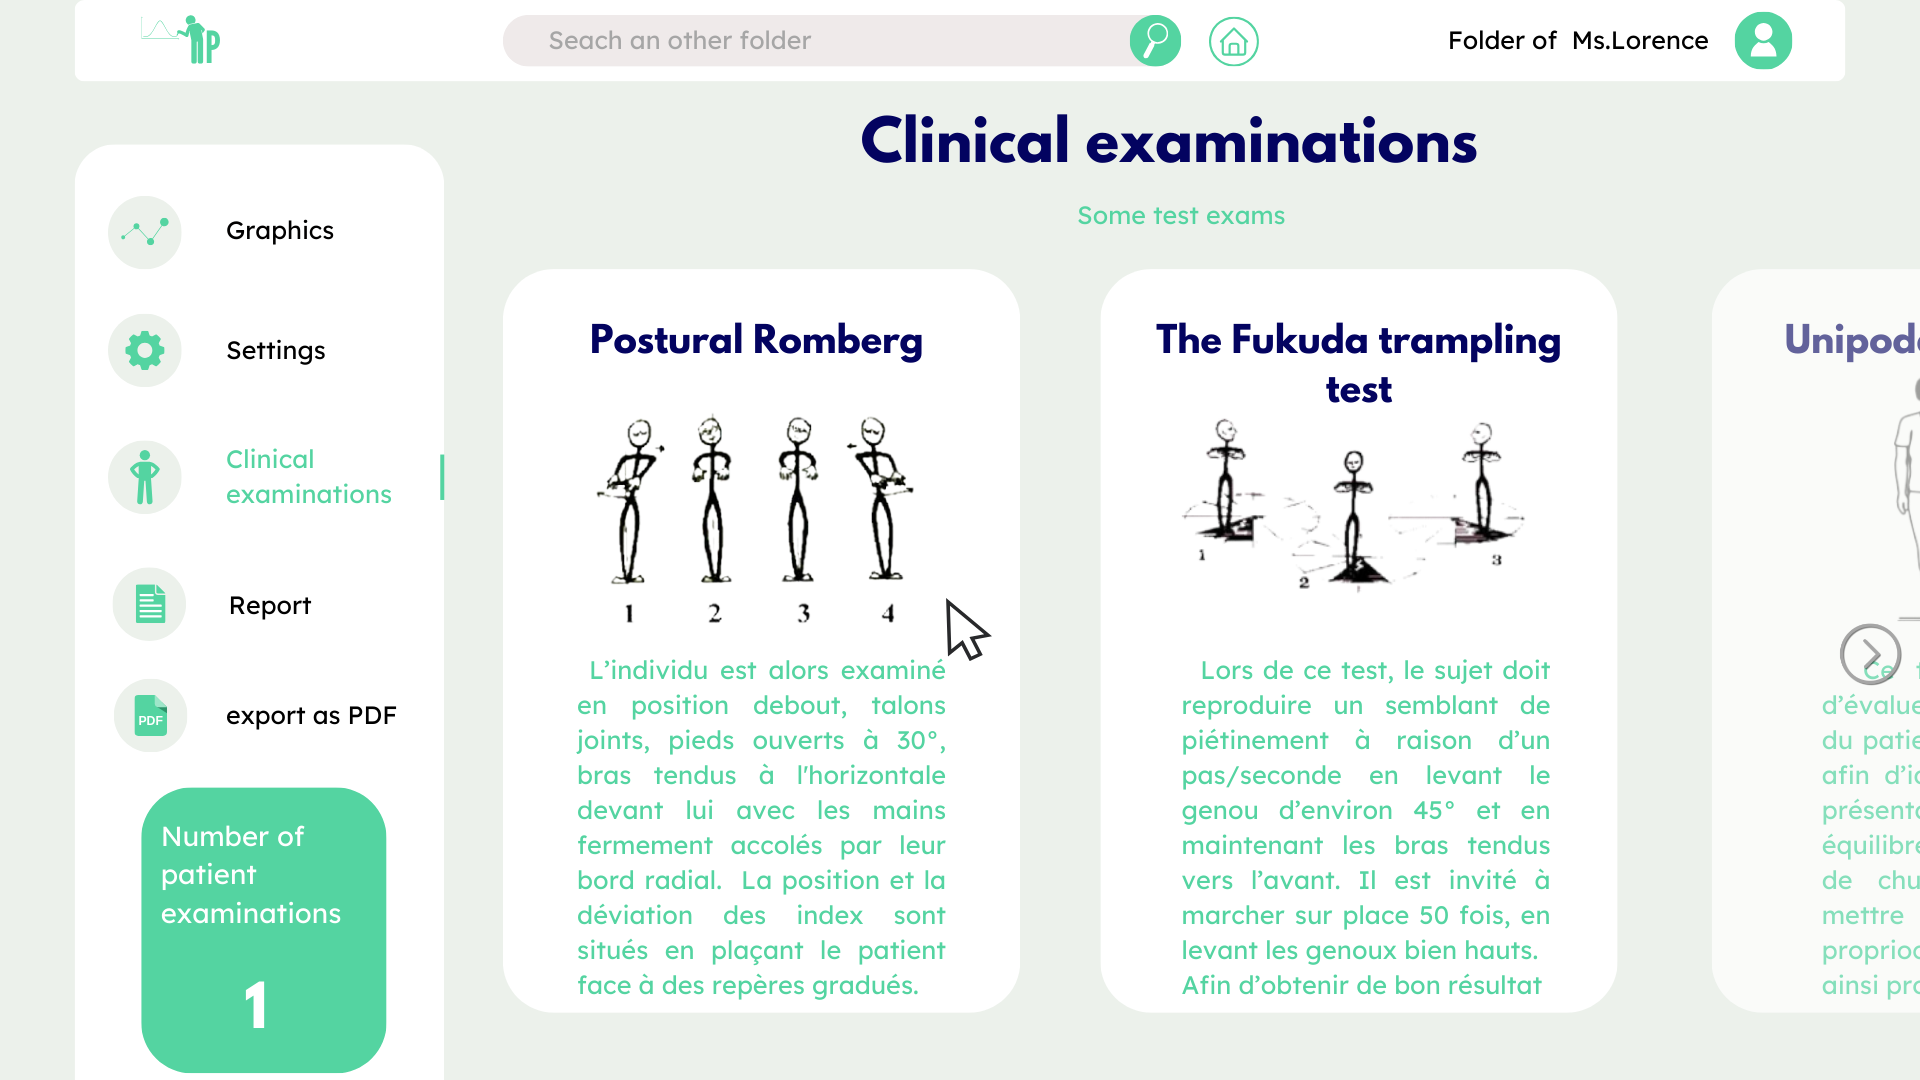
\includegraphics[width=\textwidth]{images/Prototype/11.png}
        \caption*{11}
    \end{minipage}
    \begin{minipage}{0.3\textwidth}
        \centering
        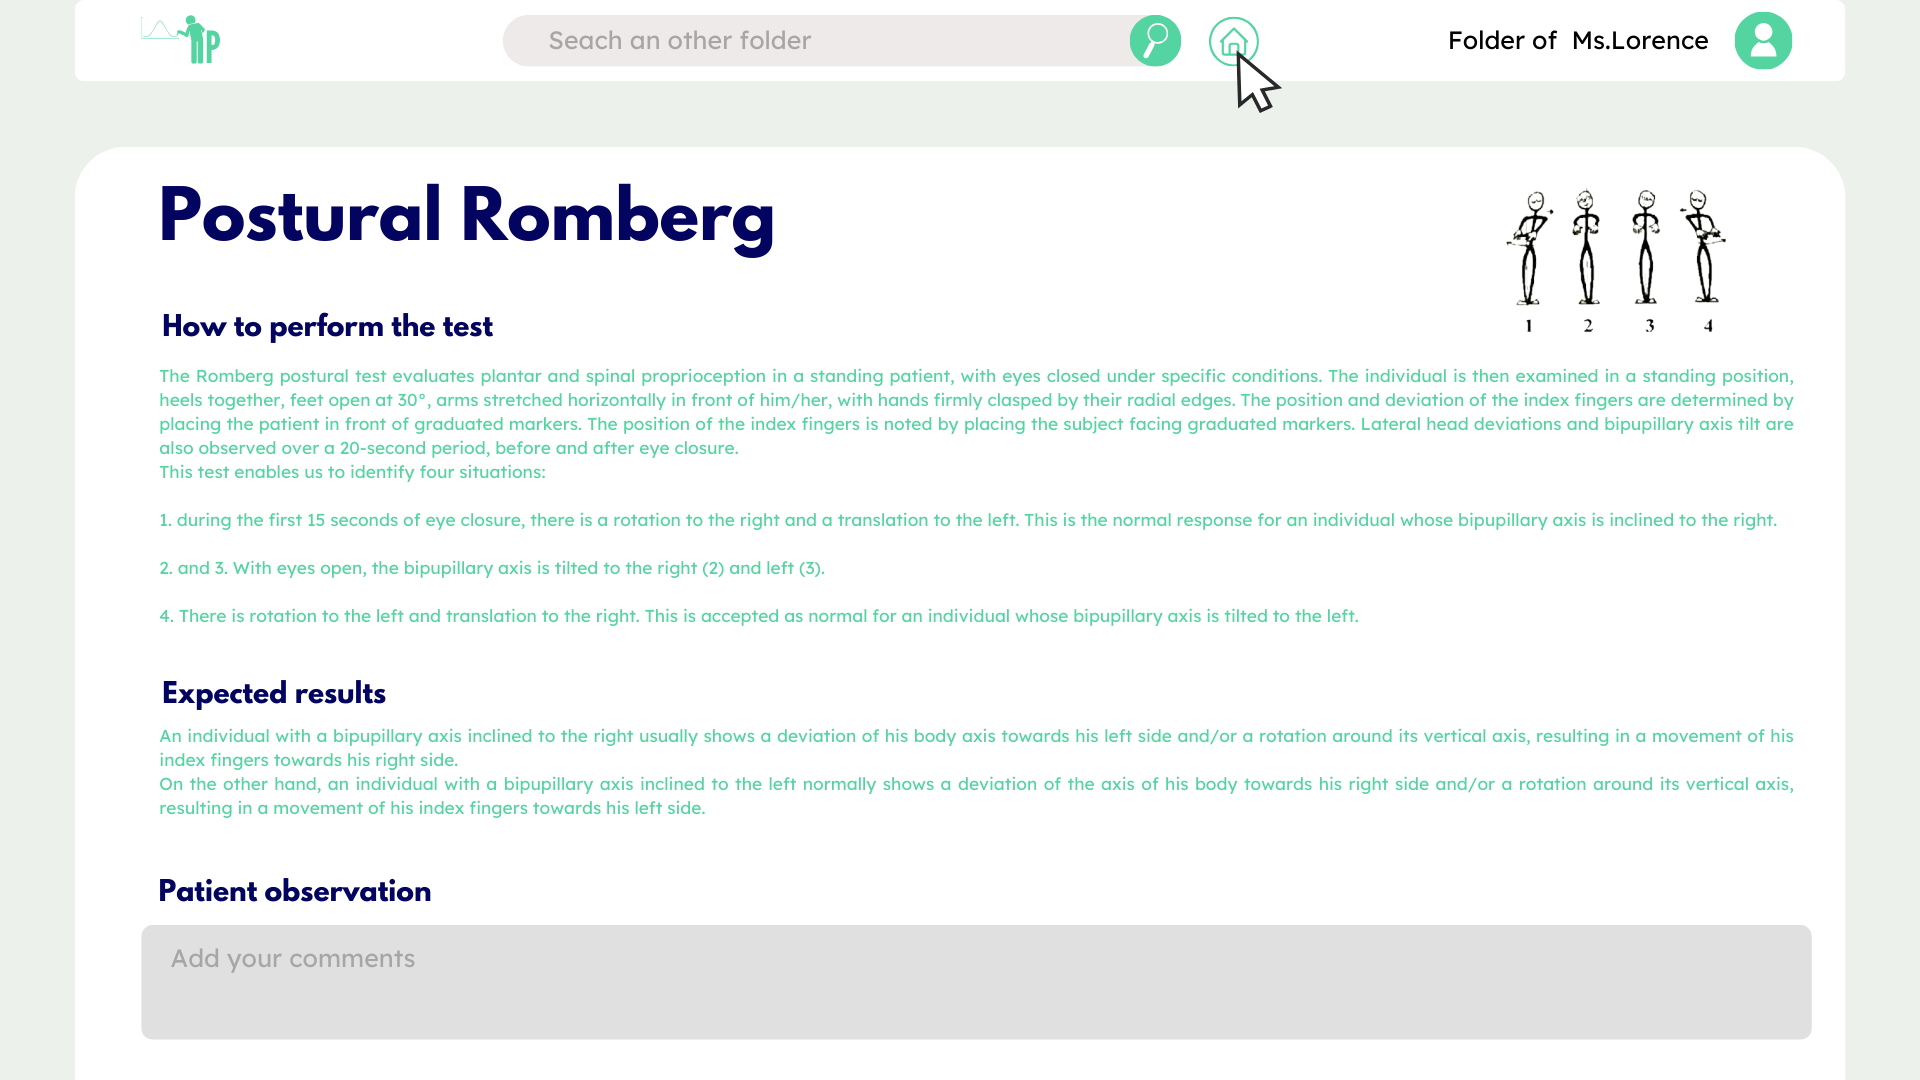
\includegraphics[width=\textwidth]{images/Prototype/12.png}
        \caption*{12}
    \end{minipage}
    \begin{minipage}{0.3\textwidth}
        \centering
        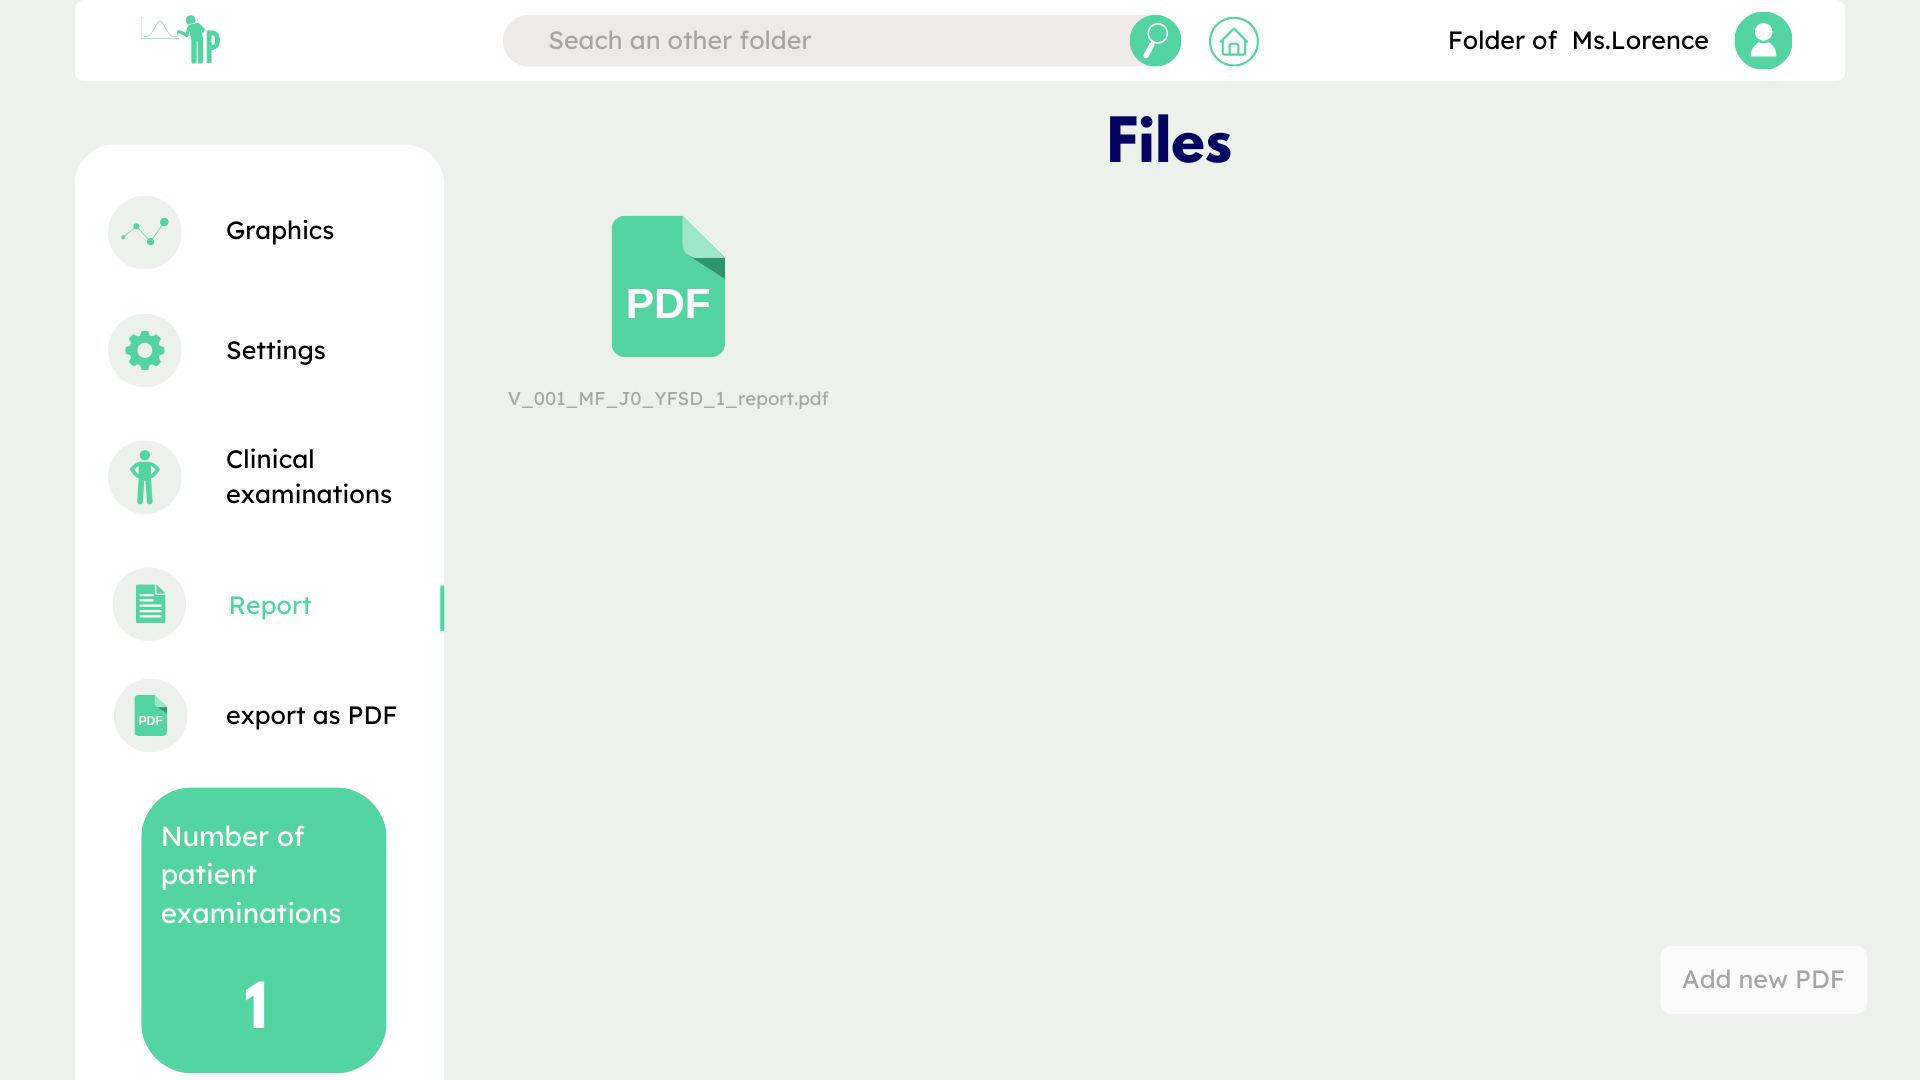
\includegraphics[width=\textwidth]{images/Prototype/13.png}
        \caption*{13}
    \end{minipage}
    \begin{minipage}{0.3\textwidth}
        \centering
        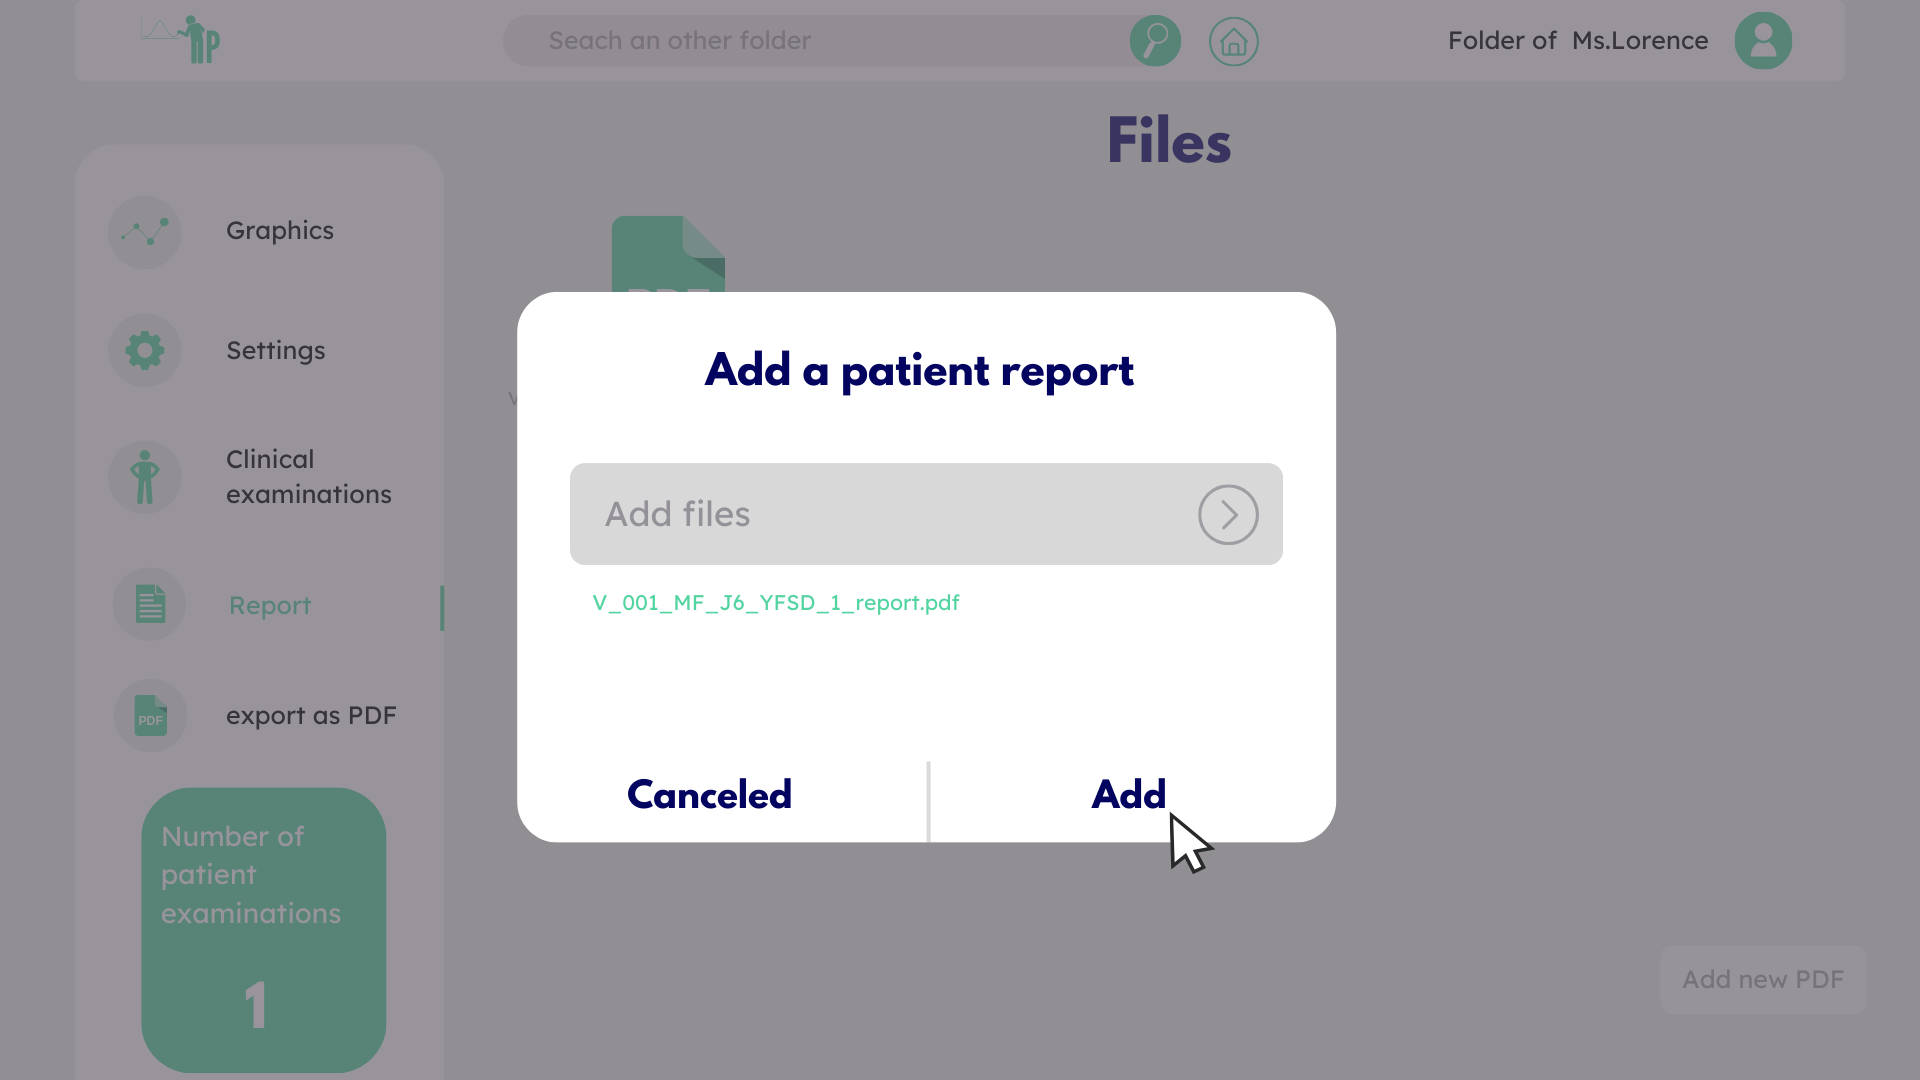
\includegraphics[width=\textwidth]{images/Prototype/14.png}
        \caption*{14}
    \end{minipage}
    \begin{minipage}{0.3\textwidth}
        \centering
        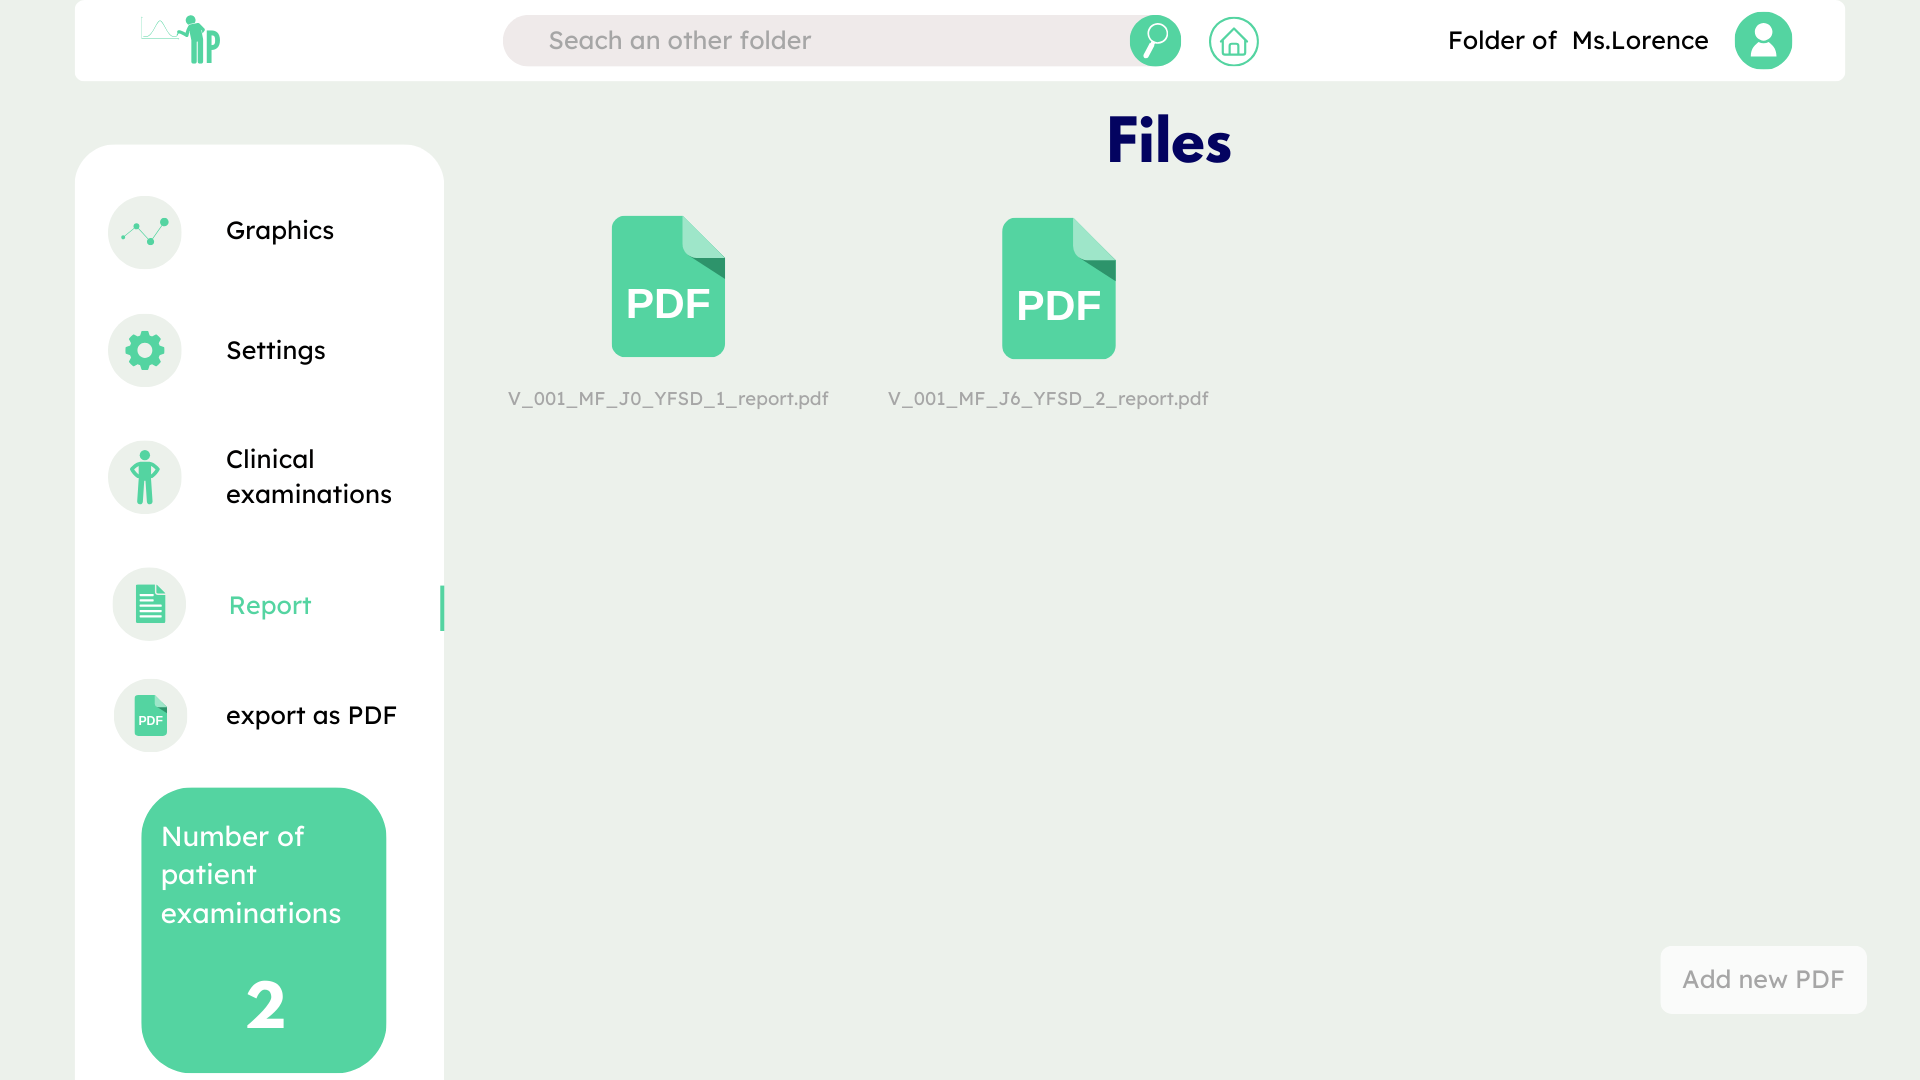
\includegraphics[width=\textwidth]{images/Prototype/15.png}
        \caption*{15}
    \end{minipage}
    \label{fig:plateforme_imaginee}
\end{figure}
